%%=============================================================================
%% LaTeX sjabloon voor bachelorproef, HoGent Bedrijf en Organisatie
%% Opleiding Toegepaste Informatica
%%=============================================================================

\documentclass[fleqn,a4paper,12pt]{book}

%%=============================================================================
%% LaTeX sjabloon voor de bachelorproef, HoGent Bedrijf en Organisatie
%% Opleiding toegepaste informatica
%%
%% Structuur en algemene vormgeving. Meestal hoef je hier niets te wijzigen.
%%
%% Vormgeving gebaseerd op "The Legrand Orange Book", version 2.0 (9/2/15)
%% door Mathias Legrand (legrand.mathias@gmail.com) met aanpassingen door
%% Vel (vel@latextemplates.com). Het oorspronkelijke template is te vinden op
%% http://www.LaTeXTemplates.com
%%
%% Aanpassingen voor HoGent toegepaste informatica: 
%%   Bert Van Vreckem <bert.vanvreckem@hogent.be>
%% Licentie: 
%%   CC BY-NC-SA 3.0 (http://creativecommons.org/licenses/by-nc-sa/3.0/)
%%=============================================================================

%%-----------------------------------------------------------------------------
%% Packages
%%-----------------------------------------------------------------------------

\usepackage[top=3cm,bottom=3cm,left=3cm,right=3cm,headsep=10pt,a4paper]{geometry} % Page margins
\usepackage[utf8]{inputenc}  % Accenten gebruiken in tekst (vb. é ipv \'e)
\usepackage{amsfonts}        % AMS math packages: extra wiskundige
\usepackage{amsmath}         %   symbolen (o.a. getallen-
\usepackage{amssymb}         %   verzamelingen N, R, Z, Q, etc.)
\usepackage[english,dutch]{babel}    % Taalinstellingen: woordsplitsingen,
                             %  commando's voor speciale karakters
                             %  ("dutch" voor NL)
\usepackage{iflang}
\usepackage{eurosym}         % Euro-symbool €
\usepackage{geometry}
\usepackage{graphicx}        % Invoegen van tekeningen
\graphicspath{{img/}}       % Specifies the directory where pictures are stored
\usepackage{tikz}            % Required for drawing custom shapes
\usepackage[pdftex,bookmarks=true]{hyperref}
                             % PDF krijgt klikbare links & verwijzingen,
                             %  inhoudstafel
\usepackage{enumitem}        % Customize lists
\setlist{nolistsep}         % Reduce spacing between list items
\usepackage{listings}        % Broncode mooi opmaken
\usepackage{multirow}        % Tekst over verschillende cellen in tabellen
\usepackage{rotating}        % Tabellen en figuren roteren

\usepackage{booktabs}        % Required for nicer horizontal rules in tables

\usepackage{xcolor}          % Required for specifying colors by name
\definecolor{maincolor}{RGB}{0,147,208} % Define the main color used for 
                             % highlighting throughout the book
                             % 0, 147, 208 = officiële kleur HoGent FBO

% Paragraph style: no indent, add space between paragraphs
\setlength{\parindent}{0em}
\setlength{\parskip}{1em}

\usepackage{etoolbox}
\usepackage{titling} % Macros for title, author, etc
\usepackage{lipsum}          % Voor vultekst (lorem ipsum)

%----------------------------------------------------------------------------------------
%	FONTS
%----------------------------------------------------------------------------------------

\usepackage{avant} % Use the Avantgarde font for headings
%\usepackage{times} % Use the Times font for headings
\usepackage{mathptmx} % Use the Adobe Times Roman as the default text font together with math symbols from the Sym­bol, Chancery and Com­puter Modern fonts

\usepackage{microtype} % Slightly tweak font spacing for aesthetics
\usepackage[utf8]{inputenc} % Required for including letters with accents
\usepackage[T1]{fontenc} % Use 8-bit encoding that has 256 glyphs

%------------------------------------------------------------------------------
%	TITLE PAGE
%------------------------------------------------------------------------------

\newcommand{\inserttitlepage}{%
\begin{titlepage}
  \newgeometry{top=2cm,bottom=1.5cm,left=1.5cm,right=1.5cm}
  \begin{center}

    \begingroup
    \rmfamily
    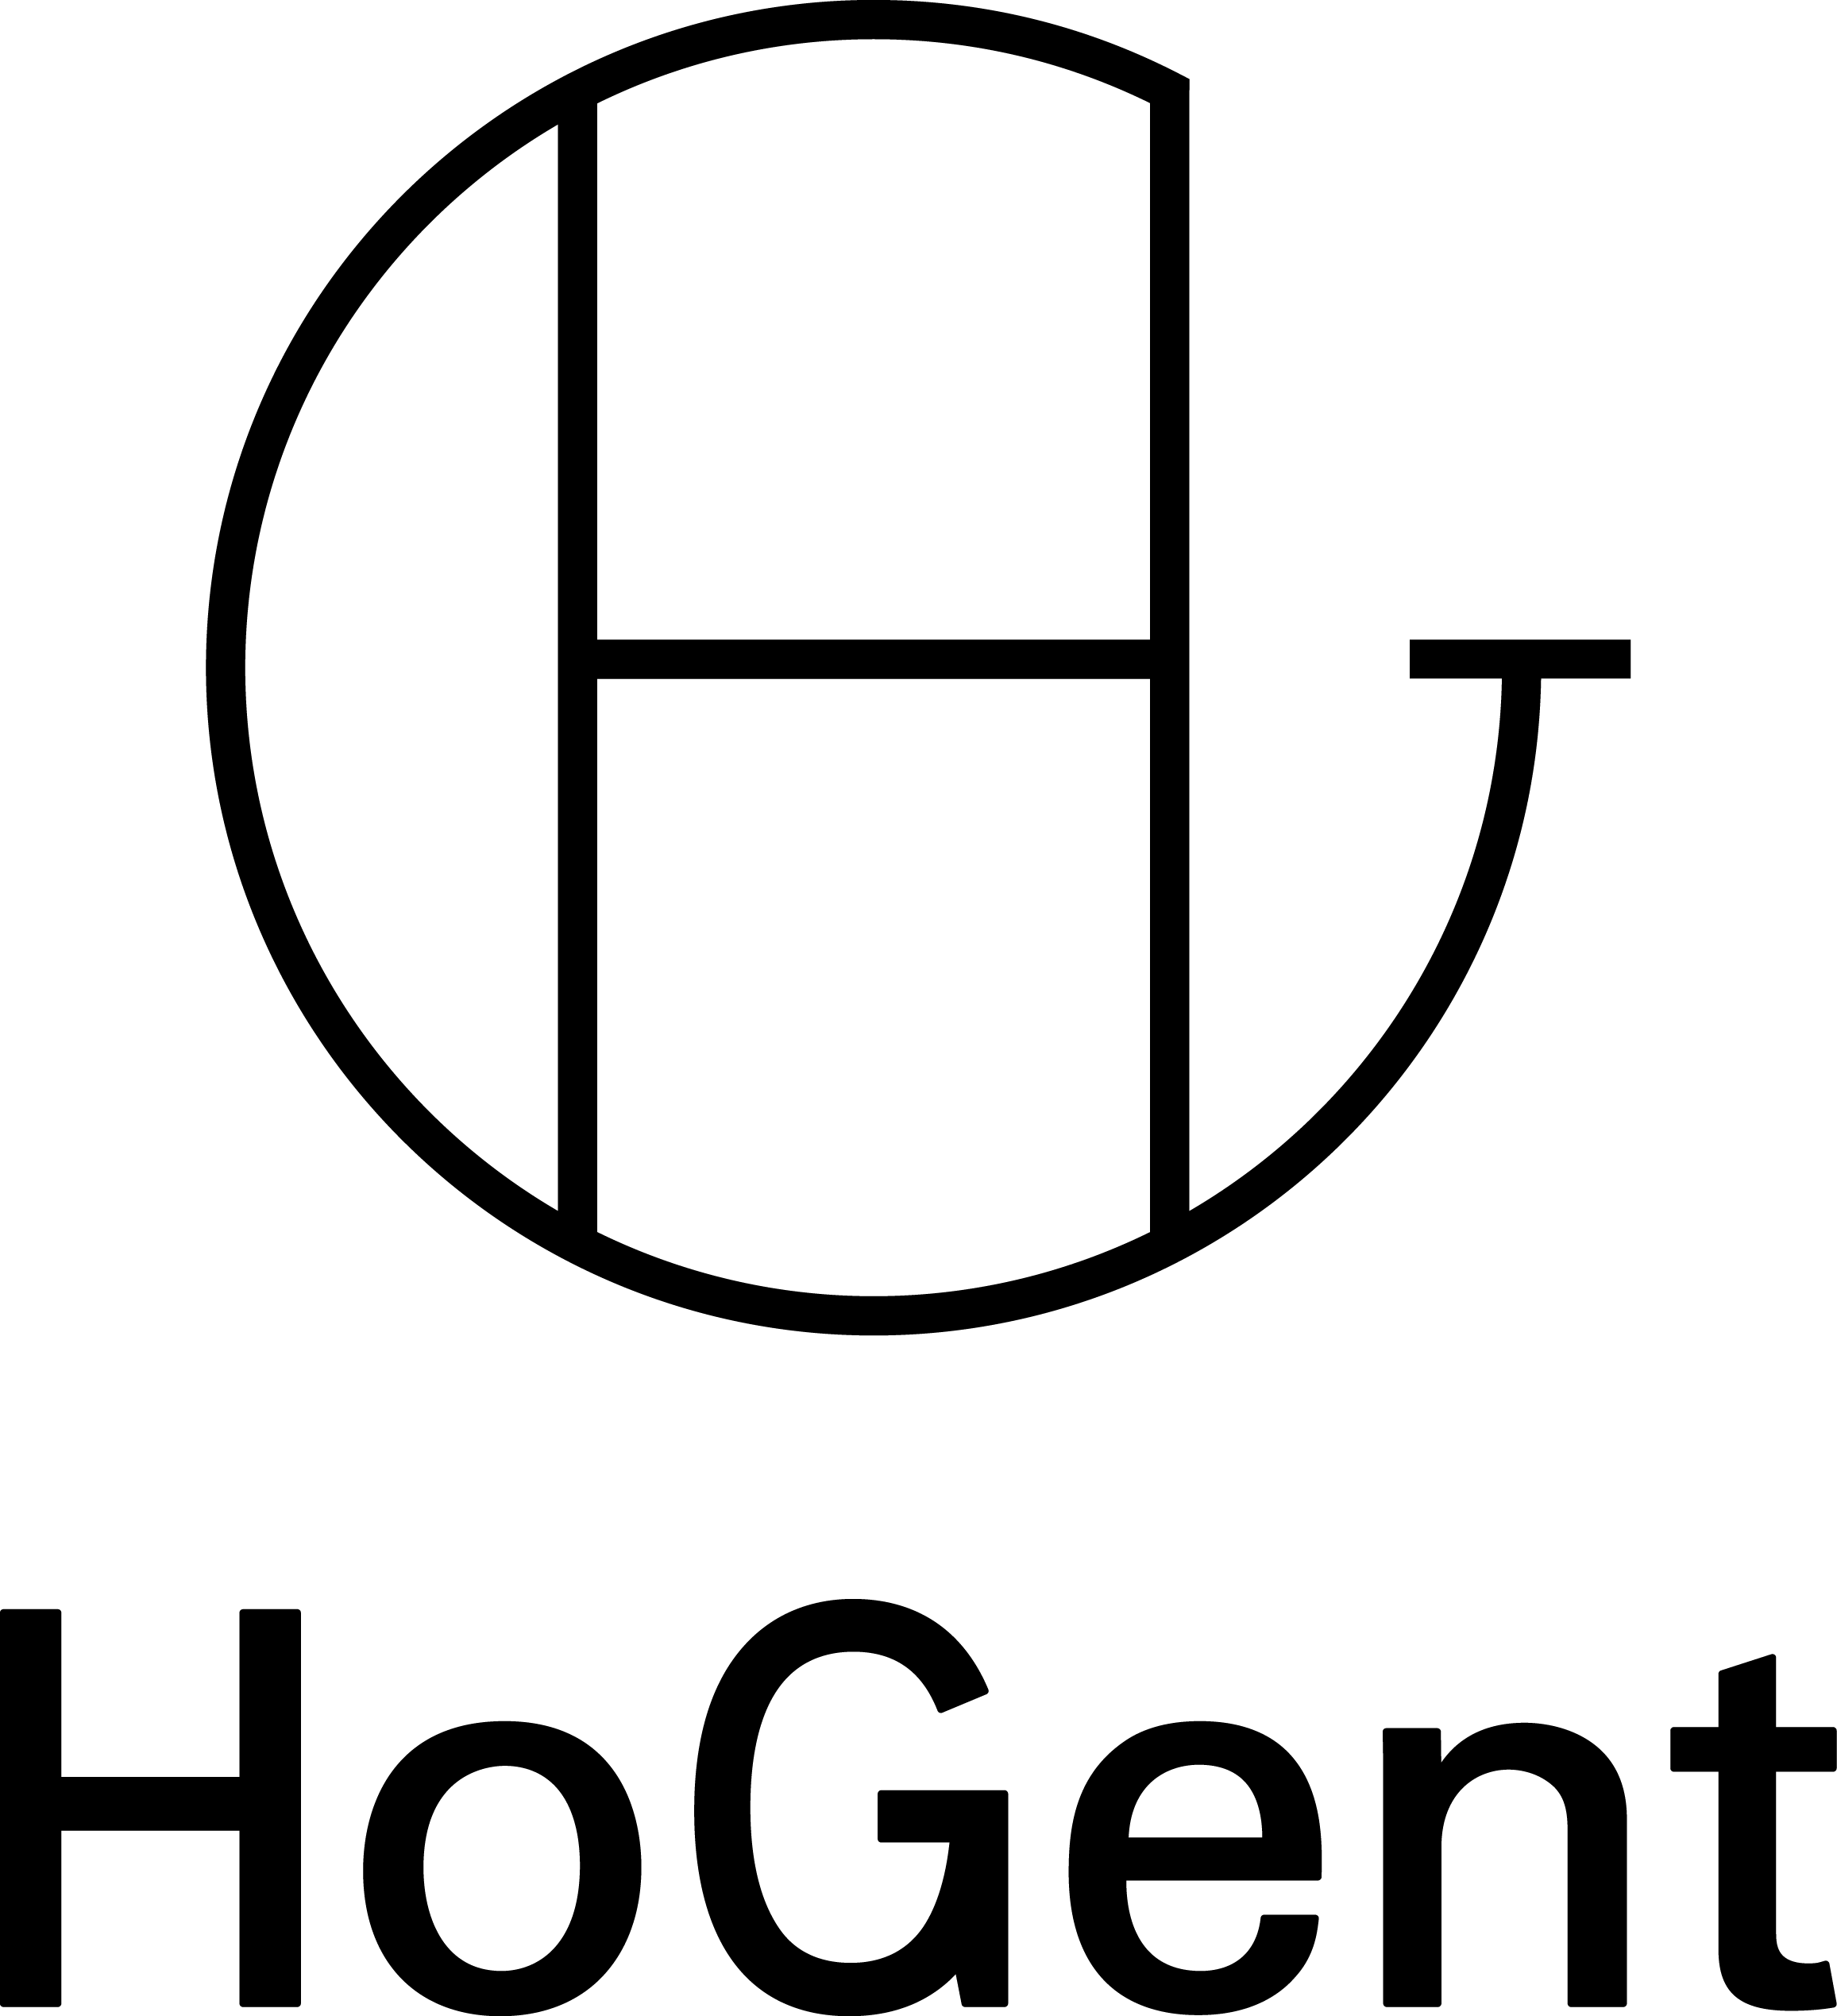
\includegraphics[width=2.5cm]{img/HG-beeldmerk-woordmerk}\\[.5cm]
    Faculteit Bedrijf en Organisatie\\[3cm]
    \titel
    \vfill
    \student\\[3.5cm]
    Scriptie voorgedragen tot het bekomen van de graad van\\professionele bachelor in de toegepaste informatica\\[2cm]
    Promotor:\\
    \promotor\\
    \ifdefempty{\copromotor}{\vspace{2.5cm}}{Co-promotor:\\\copromotor\\[2.5cm]}
    Instelling: \instelling\\[.5cm]
    Academiejaar: \academiejaar\\[.5cm]
    \ifcase \examenperiode \or Eerste \or Tweede \else Derde \fi examenperiode
    \endgroup

  \end{center}
  \restoregeometry
\end{titlepage}
  \emptypage
\begin{titlepage}
  \newgeometry{top=5.35cm,bottom=1.5cm,left=1.5cm,right=1.5cm}
  \begin{center}

    \begingroup
    \rmfamily
    \IfLanguageName{dutch}{Faculteit Bedrijf en Organisatie}{Faculty of Business and Information Management}\\[3cm]
    \titel
    \vfill
    \student\\[3.5cm]
    \IfLanguageName{dutch}{Scriptie voorgedragen tot het bekomen van de graad van\\professionele bachelor in de toegepaste informatica}{Thesis submitted in partial fulfilment of the requirements for the degree of\\professional bachelor of applied computer science}\\[2cm]
    Promotor:\\
    \promotor\\
    \ifdefempty{\copromotor}{\vspace{2.5cm}}{Co-promotor:\\\copromotor\\[2.5cm]}
    \IfLanguageName{dutch}{Instelling}{Institution}: \instelling\\[.5cm]
    \IfLanguageName{dutch}{Academiejaar}{Academic year}: \academiejaar\\[.5cm]
    \IfLanguageName{dutch}{%
    \ifcase \examenperiode \or Eerste \or Tweede \else Derde \fi examenperiode}{%
    \ifcase \examenperiode \or First \or Second \else Third \fi examination period}
    \endgroup

  \end{center}
  \restoregeometry
\end{titlepage}
}

%----------------------------------------------------------------------------------------
%	BIBLIOGRAPHY AND INDEX
%----------------------------------------------------------------------------------------

\usepackage[style=apa,backend=biber]{biblatex}
\usepackage{csquotes}
\DeclareLanguageMapping{dutch}{dutch-apa}
\addbibresource{bachproef-tin.bib} % BibTeX bibliography file
\addbibresource{../voorstel/voorstel.bib}
\defbibheading{bibempty}{}

\usepackage{calc} % For simpler calculation - used for spacing the index letter headings correctly
\usepackage{makeidx} % Required to make an index
\makeindex % Tells LaTeX to create the files required for indexing

%----------------------------------------------------------------------------------------
%	MAIN TABLE OF CONTENTS
%----------------------------------------------------------------------------------------

\usepackage{titletoc} % Required for manipulating the table of contents

\contentsmargin{0cm} % Removes the default margin

% Part text styling
\titlecontents{part}[0cm]
{\addvspace{20pt}\centering\large\bfseries}
{}
{}
{}

% Chapter text styling
\titlecontents{chapter}[1.25cm] % Indentation
{\addvspace{12pt}\large\sffamily\bfseries} % Spacing and font options for chapters
{\color{maincolor!60}\contentslabel[\Large\thecontentslabel]{1.25cm}\color{maincolor}} % Chapter number
{\color{maincolor}}
{\color{maincolor!60}\normalsize\;\titlerule*[.5pc]{.}\;\thecontentspage} % Page number

% Section text styling
\titlecontents{section}[1.25cm] % Indentation
{\addvspace{3pt}\sffamily\bfseries} % Spacing and font options for sections
{\contentslabel[\thecontentslabel]{1.25cm}} % Section number
{}
{\hfill\color{black}\thecontentspage} % Page number
[]

% Subsection text styling
\titlecontents{subsection}[1.25cm] % Indentation
{\addvspace{1pt}\sffamily\small} % Spacing and font options for subsections
{\contentslabel[\thecontentslabel]{1.25cm}} % Subsection number
{}
{\ \titlerule*[.5pc]{.}\;\thecontentspage} % Page number
[]

% List of figures
\titlecontents{figure}[0em]
{\addvspace{-5pt}\sffamily}
{\thecontentslabel\hspace*{1em}}
{}
{\ \titlerule*[.5pc]{.}\;\thecontentspage}
[]

% List of tables
\titlecontents{table}[0em]
{\addvspace{-5pt}\sffamily}
{\thecontentslabel\hspace*{1em}}
{}
{\ \titlerule*[.5pc]{.}\;\thecontentspage}
[]

%----------------------------------------------------------------------------------------
%	MINI TABLE OF CONTENTS IN PART HEADS
%----------------------------------------------------------------------------------------

% Chapter text styling
\titlecontents{lchapter}[0em] % Indenting
{\addvspace{15pt}\large\sffamily\bfseries} % Spacing and font options for chapters
{\color{maincolor}\contentslabel[\Large\thecontentslabel]{1.25cm}\color{maincolor}} % Chapter number
{}
{\color{maincolor}\normalsize\sffamily\bfseries\;\titlerule*[.5pc]{.}\;\thecontentspage} % Page number

% Section text styling
\titlecontents{lsection}[0em] % Indenting
{\sffamily\small} % Spacing and font options for sections
{\contentslabel[\thecontentslabel]{1.25cm}} % Section number
{}
{}

% Subsection text styling
\titlecontents{lsubsection}[.5em] % Indentation
{\normalfont\footnotesize\sffamily} % Font settings
{}
{}
{}

%----------------------------------------------------------------------------------------
%	PAGE HEADERS
%----------------------------------------------------------------------------------------

\usepackage{fancyhdr} % Required for header and footer configuration

\pagestyle{fancy}
\renewcommand{\chaptermark}[1]{\markboth{\sffamily\normalsize\bfseries\chaptername\ \thechapter.\ #1}{}} % Chapter text font settings
\renewcommand{\sectionmark}[1]{\markright{\sffamily\normalsize\thesection\hspace{5pt}#1}{}} % Section text font settings
\fancyhf{} \fancyhead[LE,RO]{\sffamily\normalsize\thepage} % Font setting for the page number in the header
\fancyhead[LO]{\rightmark} % Print the nearest section name on the left side of odd pages
\fancyhead[RE]{\leftmark} % Print the current chapter name on the right side of even pages
\renewcommand{\headrulewidth}{0.5pt} % Width of the rule under the header
\addtolength{\headheight}{2.5pt} % Increase the spacing around the header slightly
\renewcommand{\footrulewidth}{0pt} % Removes the rule in the footer
\fancypagestyle{plain}{\fancyhead{}\renewcommand{\headrulewidth}{0pt}} % Style for when a plain pagestyle is specified

% Removes the header from odd empty pages at the end of chapters
\makeatletter
\renewcommand{\cleardoublepage}{
\clearpage\ifodd\c@page\else
\hbox{}
\vspace*{\fill}
\thispagestyle{empty}
\newpage
\fi}

%----------------------------------------------------------------------------------------
%	THEOREM STYLES
%----------------------------------------------------------------------------------------

\usepackage{amsmath,amsfonts,amssymb,amsthm} % For math equations, theorems, symbols, etc

\newcommand{\intoo}[2]{\mathopen{]}#1\,;#2\mathclose{[}}
\newcommand{\ud}{\mathop{\mathrm{{}d}}\mathopen{}}
\newcommand{\intff}[2]{\mathopen{[}#1\,;#2\mathclose{]}}
\newtheorem{notation}{Notation}[chapter]

% Boxed/framed environments
\newtheoremstyle{maincolornumbox}% % Theorem style name
{0pt}% Space above
{0pt}% Space below
{\normalfont}% % Body font
{}% Indent amount
{\small\bf\sffamily\color{maincolor}}% % Theorem head font
{\;}% Punctuation after theorem head
{0.25em}% Space after theorem head
{\small\sffamily\color{maincolor}\thmname{#1}\nobreakspace\thmnumber{\@ifnotempty{#1}{}\@upn{#2}}% Theorem text (e.g. Theorem 2.1)
\thmnote{\nobreakspace\the\thm@notefont\sffamily\bfseries\color{black}---\nobreakspace#3.}} % Optional theorem note
\renewcommand{\qedsymbol}{$\blacksquare$}% Optional qed square

\newtheoremstyle{blacknumex}% Theorem style name
{5pt}% Space above
{5pt}% Space below
{\normalfont}% Body font
{} % Indent amount
{\small\bf\sffamily}% Theorem head font
{\;}% Punctuation after theorem head
{0.25em}% Space after theorem head
{\small\sffamily{\tiny\ensuremath{\blacksquare}}\nobreakspace\thmname{#1}\nobreakspace\thmnumber{\@ifnotempty{#1}{}\@upn{#2}}% Theorem text (e.g. Theorem 2.1)
\thmnote{\nobreakspace\the\thm@notefont\sffamily\bfseries---\nobreakspace#3.}}% Optional theorem note

\newtheoremstyle{blacknumbox} % Theorem style name
{0pt}% Space above
{0pt}% Space below
{\normalfont}% Body font
{}% Indent amount
{\small\bf\sffamily}% Theorem head font
{\;}% Punctuation after theorem head
{0.25em}% Space after theorem head
{\small\sffamily\thmname{#1}\nobreakspace\thmnumber{\@ifnotempty{#1}{}\@upn{#2}}% Theorem text (e.g. Theorem 2.1)
\thmnote{\nobreakspace\the\thm@notefont\sffamily\bfseries---\nobreakspace#3.}}% Optional theorem note

% Non-boxed/non-framed environments
\newtheoremstyle{maincolornum}% % Theorem style name
{5pt}% Space above
{5pt}% Space below
{\normalfont}% % Body font
{}% Indent amount
{\small\bf\sffamily\color{maincolor}}% % Theorem head font
{\;}% Punctuation after theorem head
{0.25em}% Space after theorem head
{\small\sffamily\color{maincolor}\thmname{#1}\nobreakspace\thmnumber{\@ifnotempty{#1}{}\@upn{#2}}% Theorem text (e.g. Theorem 2.1)
\thmnote{\nobreakspace\the\thm@notefont\sffamily\bfseries\color{black}---\nobreakspace#3.}} % Optional theorem note
\renewcommand{\qedsymbol}{$\blacksquare$}% Optional qed square
\makeatother

% Defines the theorem text style for each type of theorem to one of the three styles above
\newcounter{dummy}
\numberwithin{dummy}{section}
\theoremstyle{maincolornumbox}
\newtheorem{theoremeT}[dummy]{Theorem}
\newtheorem{problem}{Problem}[chapter]
\newtheorem{exerciseT}{Exercise}[chapter]
\theoremstyle{blacknumex}
\newtheorem{exampleT}{Example}[chapter]
\theoremstyle{blacknumbox}
\newtheorem{vocabulary}{Vocabulary}[chapter]
\newtheorem{definitionT}{Definition}[section]
\newtheorem{corollaryT}[dummy]{Corollary}
\theoremstyle{maincolornum}
\newtheorem{proposition}[dummy]{Proposition}

%----------------------------------------------------------------------------------------
%	DEFINITION OF COLORED BOXES
%----------------------------------------------------------------------------------------

\RequirePackage[framemethod=default]{mdframed} % Required for creating the theorem, definition, exercise and corollary boxes

% Theorem box
\newmdenv[skipabove=7pt,
skipbelow=7pt,
backgroundcolor=black!5,
linecolor=maincolor,
innerleftmargin=5pt,
innerrightmargin=5pt,
innertopmargin=5pt,
leftmargin=0cm,
rightmargin=0cm,
innerbottommargin=5pt]{tBox}

% Exercise box
\newmdenv[skipabove=7pt,
skipbelow=7pt,
rightline=false,
leftline=true,
topline=false,
bottomline=false,
backgroundcolor=maincolor!10,
linecolor=maincolor,
innerleftmargin=5pt,
innerrightmargin=5pt,
innertopmargin=5pt,
innerbottommargin=5pt,
leftmargin=0cm,
rightmargin=0cm,
linewidth=4pt]{eBox}

% Definition box
\newmdenv[skipabove=7pt,
skipbelow=7pt,
rightline=false,
leftline=true,
topline=false,
bottomline=false,
linecolor=maincolor,
innerleftmargin=5pt,
innerrightmargin=5pt,
innertopmargin=0pt,
leftmargin=0cm,
rightmargin=0cm,
linewidth=4pt,
innerbottommargin=0pt]{dBox}

% Corollary box
\newmdenv[skipabove=7pt,
skipbelow=7pt,
rightline=false,
leftline=true,
topline=false,
bottomline=false,
linecolor=gray,
backgroundcolor=black!5,
innerleftmargin=5pt,
innerrightmargin=5pt,
innertopmargin=5pt,
leftmargin=0cm,
rightmargin=0cm,
linewidth=4pt,
innerbottommargin=5pt]{cBox}

% Creates an environment for each type of theorem and assigns it a theorem text style from the "Theorem Styles" section above and a colored box from above
\newenvironment{theorem}{\begin{tBox}\begin{theoremeT}}{\end{theoremeT}\end{tBox}}
\newenvironment{exercise}{\begin{eBox}\begin{exerciseT}}{\hfill{\color{maincolor}\tiny\ensuremath{\blacksquare}}\end{exerciseT}\end{eBox}}
\newenvironment{definition}{\begin{dBox}\begin{definitionT}}{\end{definitionT}\end{dBox}}
\newenvironment{example}{\begin{exampleT}}{\hfill{\tiny\ensuremath{\blacksquare}}\end{exampleT}}
\newenvironment{corollary}{\begin{cBox}\begin{corollaryT}}{\end{corollaryT}\end{cBox}}

%----------------------------------------------------------------------------------------
%	REMARK ENVIRONMENT
%----------------------------------------------------------------------------------------

\newenvironment{remark}{\par\vspace{10pt}\small % Vertical white space above the remark and smaller font size
\begin{list}{}{
\leftmargin=35pt % Indentation on the left
\rightmargin=25pt}\item\ignorespaces % Indentation on the right
\makebox[-2.5pt]{\begin{tikzpicture}[overlay]
\node[draw=maincolor!60,line width=1pt,circle,fill=maincolor!25,font=\sffamily\bfseries,inner sep=2pt,outer sep=0pt] at (-15pt,0pt){\textcolor{maincolor}{R}};\end{tikzpicture}} % Orange R in a circle
\advance\baselineskip -1pt}{\end{list}\vskip5pt} % Tighter line spacing and white space after remark

%----------------------------------------------------------------------------------------
%	SECTION NUMBERING IN THE MARGIN
%----------------------------------------------------------------------------------------

\makeatletter
\renewcommand{\@seccntformat}[1]{\llap{\textcolor{maincolor}{\csname the#1\endcsname}\hspace{1em}}}
\renewcommand{\section}{\@startsection{section}{1}{\z@}
{-4ex \@plus -1ex \@minus -.4ex}
{1ex \@plus.2ex }
{\normalfont\large\sffamily\bfseries}}
\renewcommand{\subsection}{\@startsection {subsection}{2}{\z@}
{-3ex \@plus -0.1ex \@minus -.4ex}
{0.5ex \@plus.2ex }
{\normalfont\sffamily\bfseries}}
\renewcommand{\subsubsection}{\@startsection {subsubsection}{3}{\z@}
{-2ex \@plus -0.1ex \@minus -.2ex}
{.2ex \@plus.2ex }
{\normalfont\small\sffamily\bfseries}}
\renewcommand\paragraph{\@startsection{paragraph}{4}{\z@}
{-2ex \@plus-.2ex \@minus .2ex}
{.1ex}
{\normalfont\small\sffamily\bfseries}}

%----------------------------------------------------------------------------------------
%	PART HEADINGS
%----------------------------------------------------------------------------------------

% numbered part in the table of contents
\newcommand{\@mypartnumtocformat}[2]{%
\setlength\fboxsep{0pt}%
\noindent\colorbox{maincolor!20}{\strut\parbox[c][.7cm]{\ecart}{\color{maincolor!70}\Large\sffamily\bfseries\centering#1}}\hskip\esp\colorbox{maincolor!40}{\strut\parbox[c][.7cm]{\linewidth-\ecart-\esp}{\Large\sffamily\centering#2}}}%
%%%%%%%%%%%%%%%%%%%%%%%%%%%%%%%%%%
% unnumbered part in the table of contents
\newcommand{\@myparttocformat}[1]{%
\setlength\fboxsep{0pt}%
\noindent\colorbox{maincolor!40}{\strut\parbox[c][.7cm]{\linewidth}{\Large\sffamily\centering#1}}}%
%%%%%%%%%%%%%%%%%%%%%%%%%%%%%%%%%%
\newlength\esp
\setlength\esp{4pt}
\newlength\ecart
\setlength\ecart{1.2cm-\esp}
\newcommand{\thepartimage}{}%
\newcommand{\partimage}[1]{\renewcommand{\thepartimage}{#1}}%
\def\@part[#1]#2{%
\ifnum \c@secnumdepth >-2\relax%
\refstepcounter{part}%
\addcontentsline{toc}{part}{\texorpdfstring{\protect\@mypartnumtocformat{\thepart}{#1}}{\partname~\thepart\ ---\ #1}}
\else%
\addcontentsline{toc}{part}{\texorpdfstring{\protect\@myparttocformat{#1}}{#1}}%
\fi%
\startcontents%
\markboth{}{}%
{\thispagestyle{empty}%
\begin{tikzpicture}[remember picture,overlay]%
\node at (current page.north west){\begin{tikzpicture}[remember picture,overlay]%
\fill[maincolor!20](0cm,0cm) rectangle (\paperwidth,-\paperheight);
\node[anchor=north] at (4cm,-3.25cm){\color{maincolor!40}\fontsize{220}{100}\sffamily\bfseries\@Roman\c@part};
\node[anchor=south east] at (\paperwidth-1cm,-\paperheight+1cm){\parbox[t][][t]{8.5cm}{
\printcontents{l}{0}{\setcounter{tocdepth}{1}}%
}};
\node[anchor=north east] at (\paperwidth-1.5cm,-3.25cm){\parbox[t][][t]{15cm}{\strut\raggedleft\color{white}\fontsize{30}{30}\sffamily\bfseries#2}};
\end{tikzpicture}};
\end{tikzpicture}}%
\@endpart}
\def\@spart#1{%
\startcontents%
\phantomsection
{\thispagestyle{empty}%
\begin{tikzpicture}[remember picture,overlay]%
\node at (current page.north west){\begin{tikzpicture}[remember picture,overlay]%
\fill[maincolor!20](0cm,0cm) rectangle (\paperwidth,-\paperheight);
\node[anchor=north east] at (\paperwidth-1.5cm,-3.25cm){\parbox[t][][t]{15cm}{\strut\raggedleft\color{white}\fontsize{30}{30}\sffamily\bfseries#1}};
\end{tikzpicture}};
\end{tikzpicture}}
\addcontentsline{toc}{part}{\texorpdfstring{%
\setlength\fboxsep{0pt}%
\noindent\protect\colorbox{maincolor!40}{\strut\protect\parbox[c][.7cm]{\linewidth}{\Large\sffamily\protect\centering #1\quad\mbox{}}}}{#1}}%
\@endpart}
\def\@endpart{\vfil\newpage
\if@twoside
\if@openright
\null
\thispagestyle{empty}%
\newpage
\fi
\fi
\if@tempswa
\twocolumn
\fi}

%----------------------------------------------------------------------------------------
%	CHAPTER HEADINGS
%----------------------------------------------------------------------------------------

% A switch to conditionally include a picture, implemented by  Christian Hupfer
\newif\ifusechapterimage
\usechapterimagetrue
\newcommand{\thechapterimage}{}%
\newcommand{\chapterimage}[1]{\ifusechapterimage\renewcommand{\thechapterimage}{#1}\fi}%
\def\@makechapterhead#1{%
{\parindent \z@ \raggedright \normalfont
\ifnum \c@secnumdepth >\m@ne
\if@mainmatter
\begin{tikzpicture}[remember picture,overlay]
\node at (current page.north west)
{\begin{tikzpicture}[remember picture,overlay]
\node[anchor=north west,inner sep=0pt] at (0,0) {\ifusechapterimage\includegraphics[width=\paperwidth]{\thechapterimage}\fi};
\draw[anchor=west] (\Gm@lmargin,-9cm) node [line width=2pt,rounded corners=15pt,draw=maincolor,fill=white,fill opacity=0.5,inner sep=15pt]{\strut\makebox[22cm]{}};
\draw[anchor=west] (\Gm@lmargin+.3cm,-9cm) node {\huge\sffamily\bfseries\color{black}\thechapter. #1\strut};
\end{tikzpicture}};
\end{tikzpicture}
\else
\begin{tikzpicture}[remember picture,overlay]
\node at (current page.north west)
{\begin{tikzpicture}[remember picture,overlay]
\node[anchor=north west,inner sep=0pt] at (0,0) {\ifusechapterimage\includegraphics[width=\paperwidth]{\thechapterimage}\fi};
\draw[anchor=west] (\Gm@lmargin,-9cm) node [line width=2pt,rounded corners=15pt,draw=maincolor,fill=white,fill opacity=0.5,inner sep=15pt]{\strut\makebox[22cm]{}};
\draw[anchor=west] (\Gm@lmargin+.3cm,-9cm) node {\huge\sffamily\bfseries\color{black}#1\strut};
\end{tikzpicture}};
\end{tikzpicture}
\fi\fi\par\vspace*{270\p@}}}

%-------------------------------------------

\def\@makeschapterhead#1{%
\begin{tikzpicture}[remember picture,overlay]
\node at (current page.north west)
{\begin{tikzpicture}[remember picture,overlay]
\node[anchor=north west,inner sep=0pt] at (0,0) {\ifusechapterimage\includegraphics[width=\paperwidth]{\thechapterimage}\fi};
\draw[anchor=west] (\Gm@lmargin,-9cm) node [line width=2pt,rounded corners=15pt,draw=maincolor,fill=white,fill opacity=0.5,inner sep=15pt]{\strut\makebox[22cm]{}};
\draw[anchor=west] (\Gm@lmargin+.3cm,-9cm) node {\huge\sffamily\bfseries\color{black}#1\strut};
\end{tikzpicture}};
\end{tikzpicture}
\par\vspace*{270\p@}}
\makeatother

%----------------------------------------------------------------------------------------
%	HYPERLINKS IN THE DOCUMENTS
%----------------------------------------------------------------------------------------

\usepackage{hyperref}
\hypersetup{hidelinks,backref=true,pagebackref=true,hyperindex=true,colorlinks=false,breaklinks=true,urlcolor= maincolor,bookmarks=true,bookmarksopen=false,pdftitle={Title},pdfauthor={Author}}
\usepackage{bookmark}
\bookmarksetup{
open,
numbered,
addtohook={%
\ifnum\bookmarkget{level}=0 % chapter
\bookmarksetup{bold}%
\fi
\ifnum\bookmarkget{level}=-1 % part
\bookmarksetup{color=maincolor,bold}%
\fi
}
}

%----------------------------------------------------------------------------------------
%	Java source code
%----------------------------------------------------------------------------------------

% Commando voor invoegen Java-broncodebestanden (dank aan Niels Corneille)
% Gebruik:
%   \codefragment{source/MijnKlasse.java}{Uitleg bij de code}
%
% Je kan dit aanpassen aan de taal die je zelf het meeste gebruikt in je
% bachelorproef.
\newcommand{\codefragment}[2]{ \lstset{%
  language=java,
  breaklines=true,
  float=th,
  caption={#2},
  basicstyle=\scriptsize,
  frame=single,
  extendedchars=\true
}
\lstinputlisting{#1}}

% Leeg blad
\newcommand{\emptypage}{%
\newpage
\thispagestyle{empty}
\mbox{}
\newpage
}


%%---------- Documenteigenschappen --------------------------------------------
%% TODO: Vul dit aan met je eigen info:

% Je eigen naam
\newcommand{\student}{Jolan Van Impe}

% De naam van je promotor (lector van de opleiding)
\newcommand{\promotor}{Karine Van Driessche}

% De naam van je co-promotor. Als je promotor ook je opdrachtgever is en je
% dus ook inhoudelijk begeleidt (en enkel dan!), mag je dit leeg laten.
\newcommand{\copromotor}{Tim Rasschaert}

% Indien je bachelorproef in opdracht van/in samenwerking met een bedrijf of
% externe organisatie geschreven is, geef je hier de naam. Zoniet laat je dit
% zoals het is.
\newcommand{\instelling}{---}

% De titel van het rapport/bachelorproef
\newcommand{\titel}{De evolutie van IPv6 op globaal en Belgisch niveau}

% Datum van indienen (gebruik telkens de deadline, ook al geef je eerder af)
\newcommand{\datum}{28 mei 2018}

% Academiejaar
\newcommand{\academiejaar}{2017-2018}

% Examenperiode
%  - 1e semester = 1e examenperiode => 1
%  - 2e semester = 2e examenperiode => 2
%  - tweede zit  = 3e examenperiode => 3
\newcommand{\examenperiode}{2}

%%=============================================================================
%% Inhoud document
%%=============================================================================

\begin{document}

%---------- Taalselectie ------------------------------------------------------
% Als je je bachelorproef in het Engels schrijft, haal dan onderstaande regel
% uit commentaar. Let op: de tekst op de voorkaft blijft in het Nederlands, en
% dat is ook de bedoeling!

%\selectlanguage{english}

%---------- Titelblad ---------------------------------------------------------
\inserttitlepage

%---------- Samenvatting, voorwoord -------------------------------------------
\usechapterimagefalse
%%=============================================================================
%% Voorwoord
%%=============================================================================

\chapter*{Woord vooraf}
\label{ch:voorwoord}

%% TODO:
%% Het voorwoord is het enige deel van de bachelorproef waar je vanuit je
%% eigen standpunt (``ik-vorm'') mag schrijven. Je kan hier bv. motiveren
%% waarom jij het onderwerp wil bespreken.
%% Vergeet ook niet te bedanken wie je geholpen/gesteund/... heeft
Deze bachelorproef wordt beschouwd voor het afsluiten van mijn opleiding Toegepaste Informatica op HoGent. Hiermee wil ik aantonen dat ik op een zelfstandige basis een onderzoek kan voeren en afronden.

Ik heb gekozen om mijn onderwerp van mijn bachelorproef rond het nieuwere internet protocol namelijk internet protocol versie 6 te maken. Ik selecteerde dit onderwerp omdat er een grote mogelijkheid bestaat dat dit een bepaalde rol zal spelen in de toekomst van een netwerkbeheerder. Omdat dit een nieuw protocol is, heb ik hiermee zelf weinig ervaring en vond het een unieke kans om deze uitdaging aan te gaan en hierover een bachelorproef te schrijven. IPv6 is niet onbekend maar het is een protocol dat velen kennen maar weinigen volledig begrijpen, daarom wou ik onderzoeken hoe het met onze Belgische markt gesteld is en hoe deze hierop anticipeert. Ook zal dit goed aansluiten met mijn studierichting wat het nog interessanter maakt voor mezelf.
Voor dit eindresultaat te kunnen leveren, stak ik er ontzettend veel tijd in. Dankzij enkele personen heb ik deze proef met succes tot zijn eind kunnen brengen en daarom wens ik hen even te bedanken voor alle steun en hulp die ik heb gekregen tijdens deze periode.

Eerst en vooral wil ik mijn promotor bedanken namelijk mevr. Karine Van Driessche, alsook mijn co-promotor Tim Rasschaert. Dankzij de hulp van hen, heb ik deze bachelorproef tot een einde kunnen volbrengen. Vervolgens zou ik mijn familie en vriendin willen bedanken die er steeds waren tijdens de moeilijke momenten tijdens deze periode. Zij gaven mij steeds weer moed om hier volop voor te gaan.
Verder hoop ik dat het lezen van deze proef u een deugddoend gevoel zal geven.
\begin{flushright}
\textit{Jolan Van Impe,} \\
\textit{Academiejaar 2017-2018}
\end{flushright}





%%=============================================================================
%% Samenvatting
%%=============================================================================

% TODO: De "abstract" of samenvatting is een kernachtige (~ 1 blz. voor een
% thesis) synthese van het document.
%
% Deze aspecten moeten zeker aan bod komen:
% - Context: waarom is dit werk belangrijk?
% - Nood: waarom moest dit onderzocht worden?
% - Taak: wat heb je precies gedaan?
% - Object: wat staat in dit document geschreven?
% - Resultaat: wat was het resultaat?
% - Conclusie: wat is/zijn de belangrijkste conclusie(s)?
% - Perspectief: blijven er nog vragen open die in de toekomst nog kunnen
%    onderzocht worden? Wat is een mogelijk vervolg voor jouw onderzoek?
%
% LET OP! Een samenvatting is GEEN voorwoord!

%%---------- Nederlandse samenvatting -----------------------------------------
%
% TODO: Als je je bachelorproef in het Engels schrijft, moet je eerst een
% Nederlandse samenvatting invoegen. Haal daarvoor onderstaande code uit
% commentaar.
% Wie zijn bachelorproef in het Nederlands schrijft, kan dit negeren, de inhoud
% wordt niet in het document ingevoegd.

\IfLanguageName{english}{%
\selectlanguage{dutch}
\chapter*{Samenvatting}
%%\lipsum[1-4]
\selectlanguage{english}
}{}

%%---------- Samenvatting -----------------------------------------------------
% De samenvatting in de hoofdtaal van het document

\chapter*{\IfLanguageName{dutch}{Samenvatting}{Abstract}}

%%\lipsum[1-4]

Dit onderzoek zal gaan over de evolutie en adoptie van IPv6 op de Belgische markt. Het nieuwe internet protocol en de opvolger van IPv4. In 2012 was al bekend gemaakt dat het einde van de beschikbare adressen er zat aan te komen en dat er hiervoor een opvolger nodig was. Daarom werd , alsook in 2012, dag van IPv6 uitgeroepen. Hiermee was de opvolger direct voorgesteld en bekroond als officiële vervanger van IPv4. Momenteel is het 6 jaar later en is er nog niet veel meer sprake geweest van IPv6 of een effective overgang naar IPv6. Daarom zal dit onderzoek zich verdiepen in de hedendaagse adoptie van IPv6.

Er zal onderzocht worden waarom IPv6 er is gekomen en wat de positieve punten zijn aan dit protocol. Wat de verschillen zijn tussen IPv4 en IPv6, specifiek gericht op de headers van beide protocollen. Verder in deze scriptie zal er onderzocht worden wat mogelijke tunneltechnieken zijn en hoe de communicatie tussen beide protcollen kan verlopen.

Om op de meeste onderzoeksvragen een antwoord te vinden, zal er aangetoond worden wat de situatie is van IPv6 en hoe de wereld, bedrijven en ISP's zich hierop aanpassen. Hoe de overschakeling al dan niet positief aan verlopen. Na het lezen van deze scriptie zal men een beter inzicht moeten hebben over de huidige situatie en waarom deze nog niet zo hoog scoort. Ook België zal nader onderzocht worden over de hoe de Belgische bedrijven zich aanpassen en wat hun ondervinden zijn en wat men kan doen om te adoptiegroei te vergroten.







%---------- Inhoudstafel ------------------------------------------------------
\pagestyle{empty} % No headers
\tableofcontents % Print the table of contents itself
\cleardoublepage % Forces the first chapter to start on an odd page so it's on the right
\pagestyle{fancy} % Print headers again

%---------- Lijst figuren, afkortingen, ... -----------------------------------

% Indien gewenst kan je hier een lijst van figuren/tabellen opgeven. Geef in
% dat geval je figuren/tabellen altijd een korte beschrijving:
%
%  \caption[korte beschrijving]{uitgebreide beschrijving}

\listoffigures
%\listoftables

% Als je een lijst van afkortingen of termen wil toevoegen, dan hoort die
% hier thuis. Gebruik bijvoorbeeld de ``glossaries'' package.
% https://www.sharelatex.com/learn/Glossaries

%%---------- Kern -------------------------------------------------------------

%%=============================================================================
%% Inleiding
%%=============================================================================

\chapter{Inleiding}
\label{ch:inleiding}

Dankzij de groei van het internet, internetgebruikers, Internet Of Things en aantal mensen op aarde zijn er steeds meer apparaten verbonden met het internet. Dit zorgt voor de steeds verdere uitputting van IPv4 protocol. Het tekort aan beschikbare IPv4 adressen komt steeds dichterbij en de laatste /8 blok is vrijgegeven. Dit wil zeggen dat het einde van IPv4 nadert. De reeds gelanceerde opvolger, IPv6, zal de problemen van IPv4 moeten oplossen. Hierdoor is er een onderzoek nodig naar de werking en verschillen van IPv6. Verder zal er aangetoond worden wat de huidige stand van zaken is over de adoptie van IPv6 en hoever deze al staat.

\section{Probleemstelling}
\label{sec:probleemstelling}

Dankzij deze scriptie krijgt men een duidelijk visueel zicht over hoe de momentele stand van zaken is op vlak van IPv6 en de adoptie ervan over heel de wereld. Deze zou een motivatie kunnen opleveren voor andere bedrijven de stap te laten nemen naar een IPv6 of een IPv4/IPv6 netwerk structuur. Sinds de lancering van IPv6 is er al een tijd verstreken. Daarom zal deze proef een update geven van waar de huidige situatie zich bevindt.

\section{Onderzoeksvraag}
\label{sec:onderzoeksvraag}

Enkele onderzoeksvragen die gesteld kunnen worden is hoe IPv4 en IPv6 zich met elkaar onderschijden. Wat de huidige situatie is van IPv6 op globaal niveau. Hoe goed België scoort op de adoptie van IPv6. Hoe Belgische bedrijven zich hierop gaan aanpassen. Hoe het komt dat België goed of slecht scoort en wat de bevindingen zijn van bedrijven. Alsook waarom de overschakeling niet zo vlot aan het verlopen is.

\section{Onderzoeksdoelstelling}
\label{sec:onderzoeksdoelstelling}

Om deze scriptie tot een succes te brengen is het noodzakelijk genoeg data en informatie te verkregen van bedrijven. Dankzij deze data is het mogelijk om de huidige stand van zaken voor te stellen en een beeld te scheppen hoe goed de adoptie van IPv6 aan het verlopen is.

\section{Opzet van deze bachelorproef}
\label{sec:opzet-bachelorproef}

% Het is gebruikelijk aan het einde van de inleiding een overzicht te
% geven van de opbouw van de rest van de tekst. Deze sectie bevat al een aanzet
% die je kan aanvullen/aanpassen in functie van je eigen tekst.

De rest van deze bachelorproef is als volgt opgebouwd:

In Hoofdstuk~\ref{ch:methodologie} wordt de methodologie toegelicht en worden de gebruikte onderzoekstechnieken besproken om een antwoord te kunnen formuleren op de onderzoeksvragen.

% TODO: Vul hier aan voor je eigen hoofstukken, één of twee zinnen per hoofdstuk

In Hoofdstuk~\ref{ch:h1}, in het eerste hoofdstuk zal er een inleiding gegeven worden over IPv6. Dankzij dit inleidend hoofdstuk zal er al een kennis verschaft worden die interessant kan zijn voor de rest van de scriptie. Alsook worden hierin de basiselementen uitgelegd over IPv6.

In Hoofdstuk~\ref{ch:h2}, het tweede hoofdstuk bevat een gedetailleerde vergelijking tussen IPv4 en IPv6. In dit hoofdstuk zal vooral de nadruk gelegd worden op de headers van beide protocollen.

In Hoofdstuk~\ref{ch:h3}, nu IPv6 steeds populairder wordt is het ook nodig om communicatie te leggen tussen IPv4 clients en IPv6 clients. In dit hoofdstuk zullen dus enkele transitie en tunnel technieken uitgelegd worden.

In Hoofdstuk~\ref{ch:h4}, het is nu al zeker dat er een einde zal komen aan IPv4. Hierin zal verder uitgelegd worden hoe de momentele stand van zaken is voor IPv4. Hoe lang er nog te resten valt voor IPv4 en hoe de komende maanden eruit zullen zien.

In Hoofdstuk~\ref{ch:h5}, hierin zal er duidelijk de huidige adoptie grafisch voorgesteld worden op globaal niveau. Aan de hand van verschillende data en grafieken is het zeer duidelijk hierover een zicht te verkrijgen.

In Hoofdstuk~\ref{ch:h6}, in dit hoofdstuk zal er dieper gegaan worden in de adoptie op de Belgische markt ne hoe sommige bedrijven ervoor staan. Dankzij opgestelde vragen krijgt men een voorbeeld hoe de Belgische bedrijven erover denken en ervoor staan. 

In Hoofdstuk~\ref{ch:conclusie}, tenslotte, wordt de conclusie gegeven en een antwoord geformuleerd op de onderzoeksvragen. Daarbij wordt ook een aanzet gegeven voor toekomstig onderzoek binnen dit domein.


%\chapter{Stand van zaken}
\label{ch:stand-van-zaken}

% Tip: Begin elk hoofdstuk met een paragraaf inleiding die beschrijft hoe
% dit hoofdstuk past binnen het geheel van de bachelorproef. Geef in het
% bijzonder aan wat de link is met het vorige en volgende hoofdstuk.

% Pas na deze inleidende paragraaf komt de eerste sectiehoofding.

Dit hoofdstuk bevat je literatuurstudie. De inhoud gaat verder op de inleiding, maar zal het onderwerp van de bachelorproef *diepgaand* uitspitten. De bedoeling is dat de lezer na lezing van dit hoofdstuk helemaal op de hoogte is van de huidige stand van zaken (state-of-the-art) in het onderzoeksdomein. Iemand die niet vertrouwd is met het onderwerp, weet er nu voldoende om de rest van het verhaal te kunnen volgen, zonder dat die er nog andere informatie moet over opzoeken \autocite{Pollefliet2011}.

Je verwijst bij elke bewering die je doet, vakterm die je introduceert, enz. naar je bronnen. In \LaTeX{} kan dat met het commando \texttt{$\backslash${textcite\{\}}} of \texttt{$\backslash${autocite\{\}}}. Als argument van het commando geef je de ``sleutel'' van een ``record'' in een bibliografische databank in het Bib\TeX{}-formaat (een tekstbestand). Als je expliciet naar de auteur verwijst in de zin, gebruik je \texttt{$\backslash${}textcite\{\}}.
Soms wil je de auteur niet expliciet vernoemen, dan gebruik je \texttt{$\backslash${}autocite\{\}}. In de volgende paragraaf een voorbeeld van elk.

\textcite{Knuth1998} schreef een van de standaardwerken over sorteer- en zoekalgoritmen. Experten zijn het erover eens dat cloud computing een interessante opportuniteit vormen, zowel voor gebruikers als voor dienstverleners op vlak van informatietechnologie~\autocite{Creeger2009}.

%%\lipsum[7-20]

%%=============================================================================
%% Methodologie
%%=============================================================================

\chapter{Methodologie}
\label{ch:methodologie}

%% TODO: Hoe ben je te werk gegaan? Verdeel je onderzoek in grote fasen, en
%% licht in elke fase toe welke stappen je gevolgd hebt. Verantwoord waarom je
%% op deze manier te werk gegaan bent. Je moet kunnen aantonen dat je de best
%% mogelijke manier toegepast hebt om een antwoord te vinden op de
%% onderzoeksvraag.

%%\lipsum[21-25]

In dit hoofdstuk zal er besproken worden welke methodes en manieren van werking er gehandhaafd werd voor uitschrijven van deze proef. Vervolgens zal er ook een duidelijke overzicht getoond worden wat men juist van elk hoofdstuk kan verwachten.

\section{Gehanteerde methodiek}

Het onderzoek is onderverdeeld in verschillende delen. In het eerste deel zal er eerder aangetoond worden wat IPv6 inhoud en hoe deze verschilt met zijn voorganger IPv4. Dit zal al een duidelijk overzicht moeten geven waarom er de noodzaak was om de overschakeling uit te voeren. Verder zijn er ook enkele transitie technieken die kunnen toegepast worden in een netwerk om mee te gaan in deze overgang. In het tweede grote deel van de proef zal er eerder een onderzoek gedaan worden naar de adoptie van IPv6 en hoe onze Belgische markt en bedrijven hierop anticiperen. Hoe IPv4 er momenteel voor staat en hoelang dit protocol nog zal overleven tot er niets anders meer is dan IPv6. Ook werden enkele vragen opgesteld en beantwoord door bedrijven over hun standpunt en visie over IPv6. 

Om deze scriptie tot een geslaagd succes te brengen, heb ik gekozen om te onderzoeken hoe Belgische bedrijven en ISP’s reageren op IPv6. Aan bedrijven zijn er enkele vragen opgesteld en beantwoord die een duidelijk overzicht geven over hoe zij erover denken, wat hun standpunt is, of er mogelijkse plannen zijn voor een uitbreiding of ze er momenteel mee aan het experimenteren zijn. Bij ISP’s was het belangrijk of hun klanten al begeleid werden met IPv6 en of hun apparatuur IPv6 ondersteunend zijn.




% Voeg hier je eigen hoofdstukken toe die de ``corpus'' van je bachelorproef
% vormen. De structuur en titels hangen af van je eigen onderzoek. Je kan bv.
% elke fase in je onderzoek in een apart hoofdstuk bespreken.

%\input{...}
%\input{...}
%...


\chapter{Inleiding tot IPv6}
\label{ch:h1}

In dit hoofdstuk wordt er een inleiding tot IPv6, de geschiedenis en ontstaan van IPv6 doornomen. Alsook zullen er nieuwe elementen besproken worden die gehandhaafd worden in IPv6 en de reden van bestaan en waarom we dit protocol nodig zullen hebben.

\section{Waarom IPv6}

IPv4 werd ontwikkeld in de vroege jaren ’70 voor het communiceren tussen onderzoekers en academici in Amerika. Op dat moment werd er geen rekening gehouden met enkele elementen zoals genoeg adressen, extra beveiliging en Quality of Service, QoS. Het protocol heeft meer dan 30 jaar overleefd en heeft een belangrijke rol gespeeld in het internetrevolutie. Maar zelfs de slimste systemen verjaren en raken uiteindelijke verouderd. Dit was zeker het geval met IPv4. Vandaag de dag staat alles verbonden met het internet en met elkaar. De enorme opkomst van webshops, IoT, mobiel apparatuur, sociale netwerken en zo voort zorgt voor meer geconnecteerde apparaten.  Deze opkomst zorgde voor het bereiken van de limiet van IPv4 en leidde tot een opvolger namelijk IPv6. 
IPv6 werd ontwikkeld door het experimenteren met IPv4. Hierdoor werd al snel opgemerkt dat er geen limieten meer mochten zijn maar meer flexibiliteit en schaalbaarheid. IPv6 zorgde daarom voor de grote groei van het internetgebruik, mobiliteit en extra beveiliging op vlak van end-to-end beveiliging \autocite{Hagen2014}.

\section{Geschiedenis van IPv6}

Internet Engineering Taks Force (IETF) begon in de jaren 1990 met het ontwikkelen van een opvolger voor IPv4. Al snel werd er een oplossing voor de gelimiteerde tekortkomingen gezocht en extra functionaliteit toegewezen. Daarom lanceerde IETF, Internet Protocol Next Generation (IPng) zone in de jaren 1993. Dit werd gebruikt voor het onderzoeken van voorstellen en aanbevelingen van verdere procedures \autocite{Hagen2014}.

Op de Toronto IETF meeting in 1994 werd er het nieuwe protocol namelijk IPv6 voorgesteld. De bestuurders richtte een Address Lifetime Expectation (ALE) werkgroep op om na te gaan of de geschatte levenstijd van IPv4 IETF genoeg tijd gaf om een oplossing te vinden met nieuwe functionaliteit, of er enkel tijd over was om het adres probleem aan te gaan. ALE had op basis van toenmalig beschikbare statistieken geschat dat de uitputting van IPv4 plaats zou vinden tussen het jaar 2005 en 2011. Later in 1994 werd IPv6 goedgekeurd door de Internet Engineering Steering Groep \autocite{Hagen2014}.

Eén van de grootste uitdagen maar ook opportuniteiten van IPv6 is de herontwikkeling van netwerken in de toekomst. Dit is waar bedrijven hun grootse aandacht aan zouden moeten vestigen bij het overstappen naar een IPv6 netwerk. Zodanig er geen oude concepten worden meegenomen naar een nieuw protocol. Daarom is het belangrijk om bij de integratie volledig de architectuur te herstructureren \autocite{Hagen2014}. 

\section{Nieuwigheden in IPv6}

Bij de vernieuwde apparaten zal IPv6 steeds beschikbaar zijn voor configuratie. Als dit bij oudere toestellen nog niet het geval is, dan kan dit vaak via software upgrades. Enkele nieuwigheden bij IPv6 is een uitgebreid adres lengte, autoconfiguratie, het formaat van de header is eenvoudiger opgesteld en verbeterde steun voor extra opties en extensies \autocite{Hagen2014}.

\subsection{Uitgebreid adres lengte}

Het adresformaat bevat 128 bits, dit rekent uit op meer dan 340 biljoen verschillende adressen. Dit wil ook zeggen dat er meer adressen beschikbaar zijn dan korrels zand op de aarde. Dit zou het tekort aan adressen voor eens en voor altijd moeten oplossen \autocite{Hagen2014}.

\subsection{Autoconfiguratie}

Een nieuwe functionaliteit is het Stateless Address Autoconfiguration (SLAAC) mechanisme. Dit mechanisme zal ervoor zorgen dat het connecteren efficiënter zal verlopen bij vooral mobiele apparaten zoals smartphones wanneer ze zich in een onbekend netwerk bevinden. Dit zou het werk van een netwerk engineer moeten vergemakkelijken \autocite{Hagen2014}. 

\subsection{Eenvoudiger headerformaat}

De header van een IPv6 pakket is vereenvoudigd. De lengte zal een vaste lengte hebben van 40 bytes, wat het verwerken hiervan veel sneller maakt dan ervoor. De 40 bytes is onderverdeeld in twee maal 16 bytes voor het bestemmingsadres en bronadres en nog 8 bytes voor algemene header informatie \autocite{Hagen2014}.

\subsection{Verbeterde steun voor extra opties en extensies}

IPv6 heeft de optie om extension headers toe te voegen. Deze worden enkel toegevoegd als ze nodig zijn. Dit zorgt er alweer voor om het pakket sneller te verwerken. Routingheaders, QoS en beveiliging zijn enkele headers die kunnen meegegeven worden \autocite{Hagen2014}.

\section{Hebben we IPv6 echt nodig?}

Om hierop kort te antwoorden, ja. IPv6 is een noodzaak geworden in de internetwereld. We zijn op een moment gekomen dat het aantal beschikbare IPv4 adressen steeds dichter bij de nul komt. Dit is echter niet te vermijden met de dagelijkse groei van het internet. Daarom is er de overschakeling nodig naar IPv6. IPv4 had een limiet van 4,3 miljard adressen, waardoor deze limiet al snel werd bereikt \autocite{Hagen2014}. 

\chapter{Vergelijking IPv4 met IPv6}
\label{ch:h2}

In dit hoofdstuk zal er dieper worden ingegaan op de verschillen tussen beide protocollen, specifiek de vorming van de headers. Welke aanpassingen er werden gemaakt naar aanleiding van het nieuwe internet protocol en eveneens de mogelijke effecten deze verschillen kunnen hebben. Hiermee zal er een duidelijk zicht gegeven worden waarmee er juist rekening wordt gehouden naar aanleiding van de ontwikkeling van IPv6. Dit hoofdstuk bevat dus een voorstudie naar aanleiding van de overschakeling naar IPv6.

\section{Header van IPv4 en IPv6}

Onderstaande figuur geeft een duidelijke weergave van de IPv4 en IPv6 headers. Beide hebben een duidelijk verschil naar gelang de inhoud, aantal velden en aantal gebruikte bits. Op het eerste zicht is er te zien dat een IPv6 header een eenvoudiger overzicht handhaaft. Door het minder aantal velden in de header tegenover die van IPv4. Dit maakt van IPv6 een gestroomlijnder protocol en is zo efficiënter om af te handelen. Nog een voordeel hiervan is dat een IPv6 header een vaste 40 bits header bevat in vergelijking met IPv4, waarbij een IPv4 header gebruik maakt van een variabele lengte voor zijn header. Verder in dit hoofdstuk worden de verschillende velden met elkaar vergeleken.


\begin{figure}
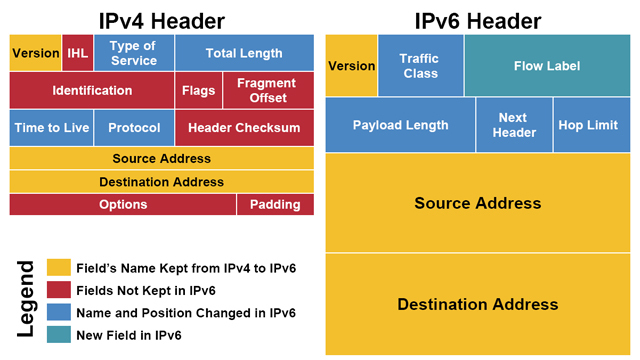
\includegraphics[width=\textwidth,height=\textheight,keepaspectratio]{vergelijking.jpg}
\centering
\caption{Vergelijking IPv4 header en IPv6 header \autocite{4vs6}}
\centering
\end{figure}

\subsection{Version Field}

Zowel IPv4 als IPv6 begint met een versie veld. Dit veld bevat de versie van het gebruikte internet protocol. Bij IPv4 zal dit de waarde 4 opleveren en voor IPv6 zal dat de waarde 6 zijn \autocite{Graziani2017}.

\subsection{IPv4 Internet Header Length (IHL) Field}

IHL is de lengte van de IPv4 header in 32-bit woorden, met optionele velden. In feite toont dit het einde van de IPv4 header en het begin van de data of payload. De minimumwaarde van dit veld is 5. Dit betekent 5 keer 32-bit woorden of 160 bits, in octetten is dit 20 bytes. Dit komt dus overeen met de minimumwaarde van een IPv4 header zonder optionele velden. Deze optionele velden kunnen de lengte van het IHL tot een maximum van 60 bytes brengen. In vergelijking met IPv6, bestaat dit veld niet meer in de nieuwe header. De reden waarom dit veld in meer van noodzaak is in de header, is omdat een IPv6 header een vaste lengte gebruikt namelijk 40 bytes. Dit zorgt ervoor dat het behandelen veel efficiënter te pas kan gaan. Ook maakt IPv6 gebruik van optionele velden maar deze hebben geen invloed op de lengte, dit behoudt de vaste lengte van de header \autocite{Graziani2017}.

\subsection{IPv4 Type of Service (ToS) en IPv6 Traffic Class Fields}

Type of Service in IPv4 en Traffic Class Fields zijn in principe dezelfde velden. Juist werd de naamgeving hiervan aangepast in IPv6. Beiden worden gebruikt om te preciseren welke soort behandeling het pakket juist zal krijgen van routers. Deze informatie zal helpen om de functies van Quality of Service (QoS) te leveren door verschillende graden van precedentie aan te bieden. Wanneer er meerdere pakketten verstuurd worden vanuit dezelfde interface dan kan de waarde in dit veld een hulp bieden voor zowel de behandeling van pakket als voor de volgorde waarin de pakketten verstuurd worden \autocite{Graziani2017}.

\subsection{IPv6 Flow Label Field}

Het flow label field wordt gebruikt om alle pakketten binnen dezelfde stroom/flow te helpen identificeren en ervoor te zorgen dat alle pakketten dezelfde behandeling krijgen van de IPv6-routers. Routers houden de individuele pakketstromen bij. Omdat de routers niet onafhankelijk de header van elk pakket hoeven te verwerken, worden deze multipakket flows efficiënter verwerkt. Echter zijn er niet veel implementaties die rekening houden met flow label. Behalve Equal Cost Multi-Path (ECMP) en Server Load Balancing (SLB). Als een flow label de waarde 0 bevat dan betekent dit dat er met het verkeer geen rekening gehouden zal worden met een flow \autocite{Graziani2017}.

\subsection{IPv4 Total Length Field, IPv6 Payload Length Field en IPv6 Jumbograms}

Het IPv4 Total Length Field is de totale lengte van het IPv4 pakket, dit wordt uitgemeten in bytes, en bevat zowel de header als de data. Het veld is een 16-bit veld en dus een maximum grootte van een IPv4 pakket is 65535 bytes. De meeste IPv4 pakketten zijn dus ook kleiner van grootte \autocite{Graziani2017}.

Het IPv6 Payload Length Field is een 16-bit veld dat de lengte in bytes van het data deel van een IPv4-pakket. Echter telt de lengte van de IPv6 header hierin niet mee en bevat het enkel de data en IPv6-extensies. Als het pakket dus extensies bevat zullen deze hierin ook meegeteld worden. Extensies worden beschouwd als een deel van de payload \autocite{Graziani2017}.

Beiden zijn met elkaar te vergelijken, behalve voor één belangrijk verschil. In het IPv4 Total Length Field bevat het de totale lengte van een IPv4-pakket, zowel data als header. Bij het IPv6 Payload Length Field is dit enkel het totaal aantal bytes van de data of payload, de header wordt hierin niet meegerekend. Daarom kan de lengte bij IPv4 verschillen door gebruik te maken van optionele velden waarbij IPv6 een vaste lengte heeft van 40 bytes \autocite{Graziani2017}.

Zoals eerder vermeld geweest, IPv4 Total Length is een 16-bit veld dat een maximum pakket grootte van 65355 bytes heeft. Deze pakketten zullen deze grootte haast nooit halen wegens de maximum transmission unit (MTU). IPv4 heeft geen optie om deze theoretische grootte te overschrijden. Daarentegen kan IPv6 zijn maximum payload wel overschrijven. Dit type van pakket wordt dan een jumbogram genoemd. Een jumbogram is een IPv6-pakket dat een grotere payload van 65535 bytes bevat. Jumbogrammen gebruiken de Jumbo Payload optie in de Hop-by-Hop extensie header. De Jumbo payload optie gebruikt een veld van 32-bit lengte groot om het verzenden van IPv6-pakketten tussen de 65536 en 4294967295 bytes toe te laten. Deze jumbogrammen worden het vaakst gebruikt bij connecties tussen supercomputers \autocite{Graziani2017}.

\subsection{IPv4 en IPv6 MTU's}

De meeste transmissie linken gebruiken een maximum pakketlengte gekend als een MTU (maximum transmission unit). Een MTU bij IPv4 en IPv6 is de totale lengte van een pakket inclusief de header \autocite{Graziani2017}. 

Echter is het nodig dat elke node de mogelijkheid heeft om een Ipv4 pakket te versturen van 68 bytes zonder verdere fragmentatie. Dit komt omdat een Ipv4 header de grootte van 60 bytes kan bevatten in lengte, waardoor er nog 8 bytes overblijven voor de payload. Daarom moet de payload een Ipv4 fragment zijn. Anders moet de payload header informatie toegevoegd krijgen voor een ander protocol, waardoor het groter dan 8 bytes zal worden. Elke IPv4 eindbestemming van het Ipv4 pakket moet een IPv4 pakket van 576 bytes kunnen ontvangen, dit kunnen ook alle fragmenten van een pakket zijn \autocite{Graziani2017}.

Bij IPv6 is het nodig dat elke link een minimum MTU van 1280 bytes heeft, met een aangeraden MTU van 1500 bytes. In vergelijk met het IPv4 protocol is dit 68 bytes \autocite{Graziani2017}.

\subsection{IPv4 Framgmentation}

Het IPv4 protocol werd eerder ontwikkeld voor een breed spectrum van transmissielinks. Als de router een IPv4 pakket ontvangt dat groter is dan de MTU van de uitgaande interface dan kan het pakket gefragmenteerd worden afhankelijk van de header van het pakket. Het kan voorvallen dat een pakket al gefragmenteerd, in meerdere pakketten, werd verzonden door de verzender. Als de finale ontvanger alle pakketten ontvangt, dan is het zijn taak om deze terug te zetten in het originele IPv4 pakket \autocite{Graziani2017}.

Fragmentatie deelt dus IPv4 pakketten in kleinere delen zodat deze kunnen doorgestuurd worden op een link dat niet de volledige grootte van het originele pakket kon verzenden. Het bestemmende apparaat heeft als taak deze ontvangen pakketten terug om te vormen naar het originele pakket. Het IPv4 Identification, Flags en Fragment Offset velden worden gebruikt om het pakket op te delen en terug samen te voegen \autocite{Graziani2017}. 

Identification veld is 16 bits groot. Elk IPv4 pakket heeft een uniek veld in het 16 bit Identification veld. Als een IPv4 pakket wordt opgesplitst in delen dan helpt dit veld om de gefragmenteerde pakketten terug samen te voegen voor de ontvanger \autocite{Graziani2017}.

Flags veld is een veld dat de grootte heeft van 3 bits. De eerste bit is 0, dit geeft aan of het gereserveerd is of niet. De tweede bit is bekend als de DF (don’t fragment) bit. Als deze de waarde 1 heeft toont dit aan dat het pakket niet gefragmenteerd is. De laatste, derde, bit is de more fragments flag. Deze bit is gebruikt om aan te tonen of dit pakket het laatste pakket is of niet. Als deze de waarde 1 heeft dan is dit pakket niet het laatste en volgen er nog. 0 geeft aan dat dit het laatste pakket is. Als een IPv4 pakket niet gefragmenteerd is dan zal deze vlag de waarde 0 bevatten \autocite{Graziani2017}.

Fragment Offset veld is een veld van 13 bits lang. Als een IPv4 pakket is gefragmenteerd dan toont dit veld aan waar het pakket gepositioneerd is en waar de data komt in delen van 8 octetten, 64 bits. De ontvanger krijgt hierdoor een beeld van waar het pakket komt tussen alle andere pakketten. Als het pakket niet gefragmenteerd is zal deze de waarde 0 hebben \autocite{Graziani2017}.

\subsection{IPv6 Fragmentation: IPv6 Source only}

Een IPv6 router zal geen fragmentering toepassen op een pakket, zoals bij IPv4 wel het geval is, enkel als het de zender is van het pakket. Zoals te zien op de afbeelding is er in de IPv6 header geen plaats gemaakt voor de velden die IPv4 gebruikt om te fragmenteren \autocite{Graziani2017}.

Als een IPv6 router een pakket ontvangt dat groter is dan de MTU uitgaande interface, dan zal de router simpelweg het pakket droppen en zal een ICMPv6 (Internet Control Message Protocol version 6) Packet Too Big bericht terug verzenden naar de zender van het pakket. Het Packet Too Big bericht bevat de MTU grootte van de link in bytes zodanig dat de zender van het pakket zijn grootte kan aanpassen en het pakket terug kan verzenden \autocite{Graziani2017}.

De data wordt vaak verzonden in series van pakketten, ook wel een packet train genoemd. Hoe groter deze pakketten zijn, hoe minder pakketten er zullen verstuurd moeten worden. Daarom is het aangeraden om de grootte zo hoog mogelijk te maken zodat alle links, van zender naar ontvanger, deze ondersteunen. Dit wordt ook de Path MTU (PMTU) genoemd. Hiervoor kan een apparaat een PMTU Discovery doen om de laagste MTU link te achterhalen \autocite{Graziani2017}.

\subsection{IPv4 Protocol en IPv6 Next Header Fields}

Het IPv4 Protocol veld toont het protocol aan dat gebruikt wordt in de data portie van het IPv4 pakket. Hiervoor heeft IPv6 een gelijkaardig veld, het Next Header veld, dat aantoont welk type header er volgt achter de algemene IPv6 header. Ook al lijkt het gelijkaardig met het IPv4 veld, toch zijn er enkele verschillen tussen beiden \autocite{Graziani2017}.

Dezelfde waarden die gebruikt worden in het IPv4 Protocol veld zijn terug te vinden in het IPv6 Next Header veld, buiten dat er bij IPv6 nog extra waarden mogelijk zijn. De meest voorkomen waarde voor beiden is voor TCP de waarde 6 en voor UDP 17 \autocite{Graziani2017}.

Als er enkel een IPv6 header is en geen extra header meer volgt, dan zal het IPv6 Next Header veld de waarde van het protocol weergeven dat wordt gebruikt in de data portie van het IPv6 pakket. Dit is dus hetzelfde voor het IPv4 Protocol veld \autocite{Graziani2017}.

\subsection{IPv4 Time To Live (TTL) en IPv6 Hop Limit Fields}

De IPv4 Time To Live (TTL) en IPv6 Hop Limit velden zorgen ervoor dat pakketten niet eindeloos blijven rondgaan in netwerken, zoals routingloops. Deze velden worden steeds verminderd door 1 als het pakket een router passeert. Als het veld de waarde 0 bereikt dan wordt het pakket weggegooid en een ICMPv4 of ICMPv6 Time Exceeded bericht verstuurd naar de zender van het pakket \autocite{Graziani2017}. 

Van IPv4 naar IPv6, was het TTL veld verandert naar het Hop Limit veld. Het IPv4 TTL veld was eigenlijk bedoelt om het maximum aantal tijd dat het pakket mag ronddolen in een netwerk en niet het aantal hops met routers. Deze tijd wordt berekend in seconden. Het maximum is 255 seconden of 4.25 minuten. In plaats van deze tijd te berekenen gaan de routers het IPv4 TTL veld verminderen met 1, hierdoor worden het aantal van hops aangekaart \autocite{Graziani2017}.

\subsection{Checksums: IPv4, TCP en UDP}

Een checksum in de IPv4 header dient ervoor om na het versturen van pakketten deze te controleren op corrupte data. Dit is een 16-bit checksum die zich focust op de IPv4 header. Elke router die dit pakket passeert zal de berekening doen van de checksum en controleren. Als deze dan gefaald of fout is zal de router het pakket verwijderen \autocite{Graziani2017}.

In IPv6 is er geen checksum in de IPv6 header. De checksum is er bewust uitgelaten omdat layer 2 data link technologie, zoals ethernet, een eigen checksum en error controle hebben. Alsook TCP en UDP hebben hun eigen checksums. Dit maakt een extra checksum op layer 3 niveau overbodig en redundant \autocite{Graziani2017}.

Omdat er geen checksum is toegevoegd in IPv6 zal de UDP checksum wel verplicht zijn bij IPv6, wat bij IPv4 niet het geval is. Dit veld dient er toe om de betrouwbaarheid van de UDP header en data te waarborgen. Bij het TCP protocol is zowel bij IPv6 als bij IPv4 de checksum een vereiste \autocite{Graziani2017}.

Checksums worden gebruikt op verschillende layers door verschillende protocollen. Een checksum zal dus controleren op mogelijk fouten die zijn opgelopen tijdens het verzenden van de data. Elk transport laag of andere bovenlaag protocol dat een IPv4 adres bevat in de berekening van de checksum moet veranderd worden voor het IPv6 te kunnen gebruiken. Deze wijziging is nodig voor het 128-bit IPv6 adres \autocite{Graziani2017}.

Wanneer TCP of UDP verzonden word over IPv6, dan bevat de checksum enkele velden namelijk IPv6 bronadres, IPv6 bestemmingsadres, de payload van de bovenlaag en de IPv6 next-header waarde \autocite{Graziani2017}.

Een wijziging aan zowel TCP als UDP voor het transporteren van IPv6 pakketten is dus nodig. Omdat beide checksums gebruik maken van de IPv6 adressen, is het dus nodig deze te herwerken voor het langere adres. Ook al zijn de adressen langer, de werkwijzen en berekeningswijze blijven dezelfde voor zowel IPv6 als IPv4 \autocite{Graziani2017}.

Bij IPv4 is er een checksum aanwezig in de header, dit maakt voor UDP de checksum overbodig. Bij IPv6 was de checksum vooral verwijdert om de snelheid van de verwerking te verbeteren. Daarom is het dus verplicht om bij TCP en UDP de checksum te gebruiken \autocite{Graziani2017}.

\subsection{IPv4 en IPv6 bronadres en bestemmingsadres velden}

Eén van de grootste veranderingen van IPv4 naar IPv6 is de lengte van het bron- en bestemmingsadres. De lengte van de adressen zijn van 32-bit adressen naar 128 bit-adressen veranderd in IPv6 \autocite{Graziani2017}. Enkele veranderingen zijn:

\begin{itemize}
    \item Het bronadres is altijd een unicast adres, bij IPv6 kan dit een link-local unicast, unique local unicast of unspecified unicast adres zijn
    \item Het bestemmingsadres kan een unicast, multicast, anycast of een broadcast adres zijn. Bij IPv6 is enkel het broadcast adres niet aanwezig
\end{itemize}


\chapter{Transitie technieken}
\label{ch:h3}

Als men spreekt over het overschakelen naar IPv6, dan is het niet de bedoeling IPv4 direct aan de kant te leggen en volledig niet meer te gebruiken. Alleen een IPv6 netwerk is meestal niet het beste idee omdat niet iedereen een diepe kennis hiervan heeft. Daarom zou het beter zijn om eerst kennis te maken met IPv6 door gebruik te maken van beide protocollen. Het probleem is dat een IPv6 netwerk niet direct kan communiceren met een IPv4. Daarom zullen er verder in dit hoofdstuk enkele methodes worden besproken over hoe IPv6 nodes met IPv4 nodes kunnen communiceren via tunneling en inkapseling en translatie. Daarbij gaan we ook het beste scenario aantonen die ideaal zou zijn om aan de slag mee te gaan in een lokaal netwerk.

\section{Tunneling en inkapseling}

Om het connecteren van IPv6 hosts over een IPv4 netwerk, zal er gebruik gemaakt worden van een IPv6 tunnel over het IPv4 netwerk.

Het IPv6 pakket dat afkomstig is van het IPv6 apparaat van de verzender zal ingekapseld worden bij het toegangspunt van de tunnel, waar het een extra IPv4 header krijgt en vervolgens als IPv4 pakket zal verstuurd worden door het IPv4 netwerk. Bij het einde van de tunnel zal de IPv4 header verwijderd worden en het pakket zal nadien als een IPv6 pakket toekomen bij het IPv6 bestemmingsapparaat. Enkele methodes die verder worden uitgelegd zijn 6in4, 6to4, 6rd, GRE, ISATAP en DS-Lite \autocite{RIPE2016}.

\begin{figure}
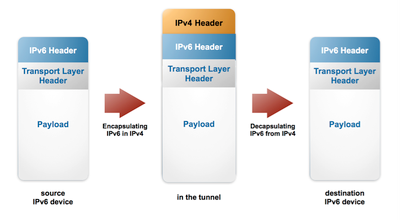
\includegraphics[width=\textwidth,height=\textheight,keepaspectratio]{Tunneling.png}
\centering
\caption{Tunneling en inkapseling \autocite{RIPE2016}}
\centering
\end{figure}

\subsection{6in4}

Als een IPv4 host, een IPv6 wilt bereiken maar geen ipv6 connectiviteit heeft thuis , is er de mogelijkheid een  6in4 tunnel op te zetten. Op het moment dat een IPv4 host een webserver via IPv6 wil bereiken is dit echter niet mogelijk. Hiervoor kan er gebruik gemaakt worden van een 6in4 tunnel. De host dient een tunnel op te zetten en gebruik te maken van een tunnelbroker. Via de tunnelbroker zal er een IPv6 adres beschikbaar zijn waarnaar de IPv6 pakketten verstuurd zullen worden. Een 6in4 tunnel zal een verzonden IPv6 pakket van de host omzetten naar een IPv4 pakket. Men zal een nieuwe IPv4 header toevoegen over de IPv6 header. Hierdoor kan het pakket verzonden worden over het IPv4 internet. Als het pakket de tunnelbroker bereikt dan zal hij op zijn moment het pakket uitpakken en de IPv4 header verwijderen. Nadien blijft enkel het oorspronkelijke IPv6 pakket over en wordt deze over het IPv6 internet verstuurd naar de webserver. Dit mechanisme is een stabiele en voorspelbare manier omdat men steeds weet naar waar het pakket zal verzonden worden. Voor een ISP is dit echter geen gangbare methode. Als een ISP gebruik zal maken van een 6in4 tunnel, dan zal deze voor iedere klant manueel een tunnel moeten aanmaken \autocite{RIPE2016}. 

\begin{figure}
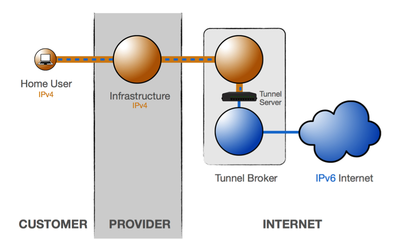
\includegraphics[width=\textwidth,height=\textheight,keepaspectratio]{6in4.png}
\centering
\caption{6in4 visualisatie \autocite{RIPE2016}}
\centering
\end{figure}

\subsection{6to4}

Doorgaans wordt 6to4 tunneling niet meer gebruikt. 6to4 is een tunneltechniek die het nadeel van de vorige mechaniek oplost, 6in4. Deze techniek is, in vergelijking met 6in4, beter schaalbaar op grotere vlakken. Hiermee zou een ISP voor al zijn klanten de techniek kunnen hanteren. Echter heeft deze methode enkele nadelen. Er kunnen zich op onverwachte momenten een lange latency veroorzaken met zeer negatieve gebruikservaringen tot gevolg. 6to4 gebruikt overal in de wereld dezelfde IPv6 en IPv4 prefix voor het begin en einde van de tunnel. Namelijk 2002::/16 voor IPv6 en 192.88.99.0/24 voor IPv4. Wanneer IPv6 bronapparaat met 6to4 tunnel een connectie wilt aangaan met een ander IPv6 apparaat over IPv4 internet, dan zal de tunnel automatisch een einde vinden zonder dat er configuratie nodig is aan de tunnel zelf. Hierdoor is de schaalbaarheid groot en dient er geen manuele configuratie meer te gebeuren. Echter heeft de eindgebruiker wel een publiek IPv4 adres nodig om de connectie succesvol tot stand te brengen. Het IPv4 tunneluitgangspunt is geïntegreerd in de bitnummers 17-48 van het 6to4 IPv6-adres. Dus het tunnelingangspunt neemt automatisch het IPv4-adres van het tunneluitgangspunt van de tunnel over van het IPv6-aders van de bestemming \autocite{RIPE2016}.

\begin{figure}
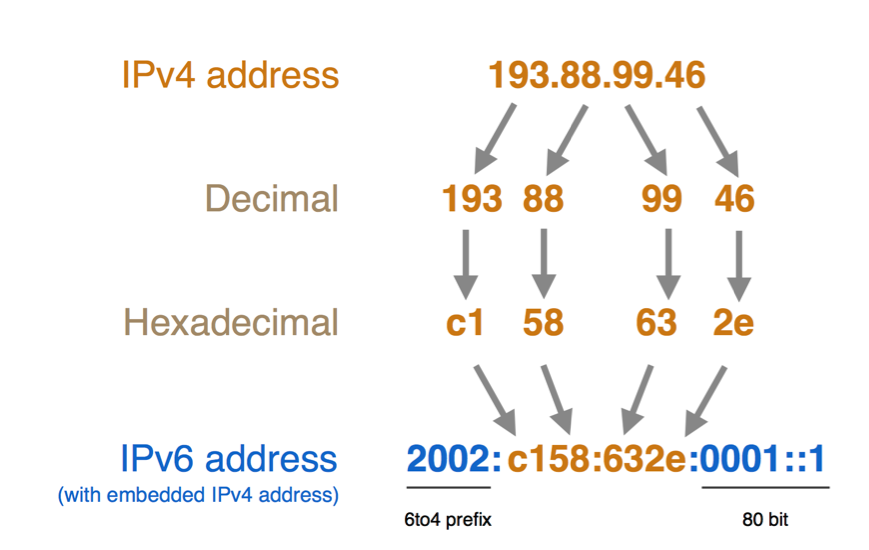
\includegraphics[width=\textwidth,height=\textheight,keepaspectratio]{6to4.png}
\centering
\caption{6to4 omzetting \autocite{RIPE2016}}
\centering
\end{figure}

Een schematische voorstelling van de verschillende delen van een 6to4 IPv6 adres is als volgt.

\begin{figure}
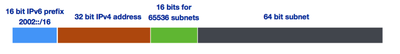
\includegraphics[width=\textwidth,height=\textheight,keepaspectratio]{6to4_2.png}
\centering
\caption{6to4 schematische voorstelling \autocite{RIPE2016}}
\centering
\end{figure}

Omdat de eindpunten van de tunnel anycasted zijn, wilt dit zeggen dat de gebruiker geen controle heeft over welke tunnel effectief gebruikt zal worden. Het terugkerende verkeer kan hierdoor ook een ander ingangspunt van een tunnel nemen wat kan leiden tot asymmetrische routes, lange latencies en onaanvaardbare wachttijden voor de gebruikers hiervan \autocite{RIPE2016}.

\begin{figure}
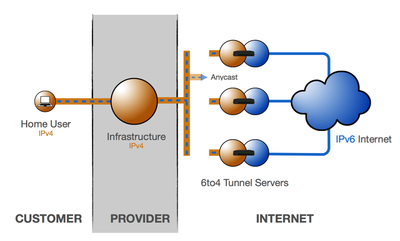
\includegraphics[width=\textwidth,height=\textheight,keepaspectratio]{6to4_3.png}
\centering
\caption{6to4 visualisatie \autocite{RIPE2016}}
\centering
\end{figure}

\subsection{6rd}

De derde methode namelijk 6rd, werd ontwikkeld om de problemen zoals lange latencies, die eigenaardig waren bij de tunneltechniek 6to4, op te lossen. Ook zal 6rd de schaalbaarheid behouden die te vinden was bij 6to4. Ondertussen is 6rd al ingevoerd bij enkele miljoenen personen \autocite{RIPE2016}. 

Het principe achter deze techniek is zeer eigenaardig aan die van 6to4. Eén van de belangrijkste verschillen is dat de IPv4 en IPv6 adresruimte van de ISP nu gebruikt zal worden voor de eindpunten van de tunnels. Dit betekent dat anycast niet langer meer gebruikt zal worden. Het verkeer wordt hierdoor symmetrisch en wordt door de ISP beheerd \autocite{RIPE2016}.

\begin{figure}
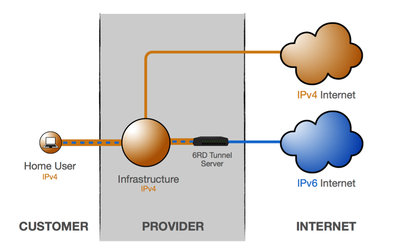
\includegraphics[width=\textwidth,height=\textheight,keepaspectratio]{6rd_1.png}
\centering
\caption{6rd visualisatie \autocite{RIPE2016}}
\centering
\end{figure}

Net zoals bij 6to4 moeten de IPv4-adressen van de tunneleindpunten in het IPv6-adres van de eindgebruiker worden geïntegreerd. Aangezien de eerste 32 bits van het IPv6-adres van het eindapparaat opgenomen zal worden door de prefix van de ISP en de tweede 32 bits gebruikt zal worden voor de IPv4 adressen van de tunneleindes. Slechts één /64 IPv6 range zal beschikbaar zijn voor elk apparaat \autocite{RIPE2016}.

\begin{figure}
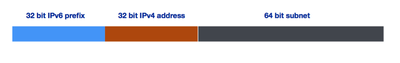
\includegraphics[width=\textwidth,height=\textheight,keepaspectratio]{6rd.png}
\centering
\caption{6rd schematische voorstelling deel 1 \autocite{RIPE2016}}
\centering
\end{figure}

Het aanvragen van een grotere toewijzing van adresruimte, /29 in plaats van een /32, zou drie extra bits betekenen. Dit komt overeen met acht IPv6-subnetten die aan elk eindapparaat kan toegewezen worden in plaats van slechts één \autocite{RIPE2016}. 

\begin{figure}
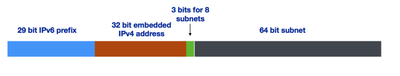
\includegraphics[width=\textwidth,height=\textheight,keepaspectratio]{6rd_2.png}
\centering
\caption{6rd schematische voorstelling deel 2 \autocite{RIPE2016}}
\centering
\end{figure}

Er is ook de mogelijkheid om te kiezen voor alleen het variabele deel van een IPv4-adres in het 6rd IPv6-adres te integreren. Als er een /21 IPv4-allocatie gebruikt wordt, dan betekent dat, dat de variabele bits, de laatste 11 bits, worden geïntegreerd in plaats van alle 32 bits van het IPv4-adres \autocite{RIPE2016}.

\begin{figure}
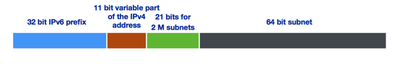
\includegraphics[width=\textwidth,height=\textheight,keepaspectratio]{6rd_3.png}
\centering
\caption{6rd schematische voorstelling deel 3 \autocite{RIPE2016}}
\centering
\end{figure}

Het combineren van beide methodes, zowel het gebruik maken van een /29 IPv6-toewijzing en het gebruik maken van de variabele bits van het IPv4 adres, geeft ons het volgende weer \autocite{RIPE2016}.

\begin{figure}
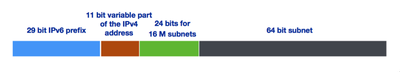
\includegraphics[width=\textwidth,height=\textheight,keepaspectratio]{6rd_4.png}
\centering
\caption{6rd schematische voorstelling deel 4 \autocite{RIPE2016}}
\centering
\end{figure}

\subsection{DS-Lite}

DS-Lite staat voor Dual Stack Lite en is vooral gebaseerd op native IPv6, tunneling en NAT (Network Address Translation).

In tegenstelling tot alle andere transitietechnieken die reeds besproken zijn, gaat DS-Lite zijn IPv4-pakketten inkapselen in IPv6-pakketten. Wat resulteert in het tunnelen van IPv4 over IPv6. Dit is precies de tegenovergestelde werking van alle vorige besproken methodes \autocite{RIPE2016}.

DS-Lite kan een IPv6-apparaat verbinding laten maken met een IPv4-apparaat en het IPv4-internet. Het voornaamste doel van DS-Lite is dat een ISP geen publiek IPv4 adres maar moet toewijzen aan een klant. In plaats daarvan worden alleen globale IPv6-adressen toegewezen \autocite{RIPE2016}.

De CPE verdeelt, hetzelfde als een NAT-apparaat, private IPv4-adressen aan klanten. In plaats van de NAT zelf laten uit te voeren gaat de CPE het IPv4-pakket inkapselen in een IPv6-pakket. De CPE maakt hierbij gebruik van zijn wereldwijde IPv6-verbinding om het pakket op een correcte manier af te leveren aan de CGN van de ISP (carrier-grade NAT) dat een openbaar IPv4-adres heeft. Het IPv6 pakket wordt op zijn beurt uitgepakt waardoor het IPv6 pakket terug naar het oorspronkelijke IPv4 pakket wordt hersteld. NAT zal nadien uitgevoerd worden op het IPv4-pakket en het pakket zal zo door het openbare IPv4-internet gestuurd worden naar zijn bestemming \autocite{RIPE2016}. 

\begin{figure}
\centering
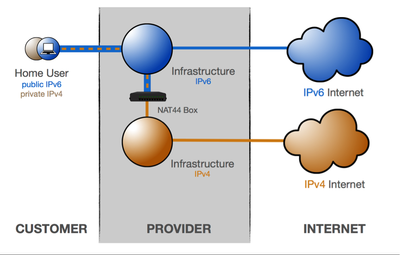
\includegraphics[width=\textwidth,height=\textheight,keepaspectratio]{dslite.png}
\caption{DS-Lite visualisatie \autocite{RIPE2016}}
\end{figure}

\subsection{Teredo}

Teredo is een per-host tunneltechniek voor het verzenden van IPv6 pakketten achter NAT apparaten via IPv4. De IPv6-pakketten worden ingepakt als een IPv4-pakket met een UDP header van het bestemmingsadres van een Teredo server met een welbekend UDP poort 3544. De algemene Teredo server voor windows is teredo.ipv6.microsoft.com. Alle tunnels naar Teredo gebruikers delen dezelfde IPv6 prefix namelijk 2001:0::/32 gevolgd door het IPv4 adres van de gebruikte Teredo Server. In het geval van Microsoft is dit 94.245.121.251 en omgezet in hexadecimaal is het 5ef5:79fb. Het adres met beide prefixen ziet er als volgt uit, 2001:0:5ef5:79fb::/64 \autocite{Vinciguerra2013}.

\begin{figure}
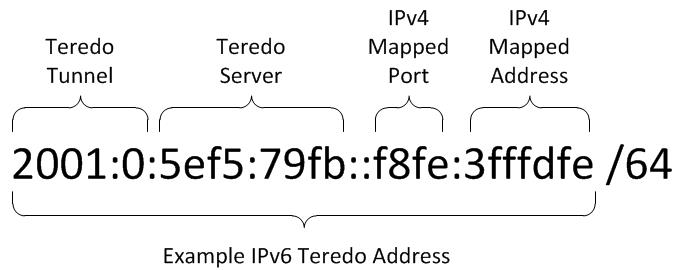
\includegraphics[width=\textwidth,height=\textheight,keepaspectratio]{teredo.jpg}
\centering
\caption{Teredo schematische voorstelling \autocite{Vinciguerra2013}}
\centering
\end{figure}

De Teredo gebruiker zal een IPv4 router soliciation versturen naar de Teredo server. Nadien zal de server de gebruiker voorzien van zijn IPv6-adres door het versleutelen van zijn IPv6-adres door het NATed bron IPv4-adres en de UDP-bronpoort naar het einde van het IPv6-adres \autocite{Vinciguerra2013}.

\begin{figure}
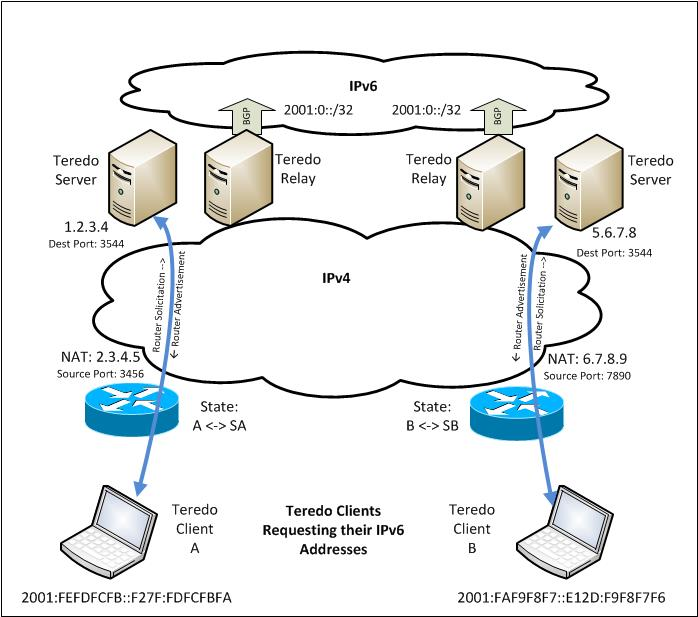
\includegraphics[width=\textwidth,height=\textheight,keepaspectratio]{teredo2.jpg}
\centering
\caption{Teredo visualisatie \autocite{Vinciguerra2013}}
\centering
\end{figure}

Het Teredo protocol is gebaseerd op een speciaal IPv6-pakket zonder payload dat een luchtbeld wordt genoemd, om door NAT apparaten te geraken. Er zijn twee soorten bubbels. Als eerst zijn er de directe bubbels, die van Teredo peer naar Teredo peer worden verstuurd. Als tweede zijn er de indirecte bubbels die door de Teredo server van de peer verstuurd worden \autocite{teredo}.

\subsection{ISATAP}

ISATAP (Intra Site Automatic Tunneling Address Protocol) is een interface die hosts kunnen gebruiken om IPv6 verkeer over een IPv4 netwerk te laten verzenden. Door het toevoegen van headers met IPv4 netwerk informatie aan het IPv6 pakket kan de gebruiker pakketten verzenden over het netwerk naar een IPv6 bestemming. Nadien kan de ontvanger van het pakket deze uitpakken tot zijn originele staat \autocite{RIPE2016}.

ISATAP is vrij eenvoudig om te herkennen. De adressen die dit protocol hanteert zijn zeer uniek geformatteerd. Een voorbeeld van een ISATAP adres is 2002:9D36:1:2:0:5EFE:192:168:12:9 \autocite{RIPE2016}.

Bij nader inzien zijn er twee opvallende delen aan het adres. Het eerste deel, 2002:9D36:1:2:0:5EFE: is geformatteerd als een typisch IPv6 adres. Het tweede deel, 192.168.12.9, is het formaat van een IPv4 adres. Het formaat hiervan bevat essentiële informatie. Ten eerste is het adres een geldig IPv6 adres waarmee IPv6 connectie mogelijk is. Vervolgens geeft de aanwezigheid van het IPv4-adres, de IPv4-informatie aan die zal gebruikt worden om het IPv6-verkeer over het IPv4-netwerk te leiden \autocite{RIPE2016}.

\begin{figure}
  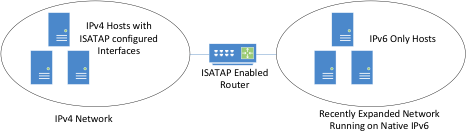
\includegraphics[width=\textwidth,height=\textheight,keepaspectratio]{isatap.png}
  \centering
  \caption{ISATAP visualisatie \autocite{RIPE2016}}
  \centering
\end{figure}

Met een ISATAP router en het configureren van ISATAP bij hosts in het IPv4 netwerk, is het mogelijk om IPv6 only hosts te laten communiceren met het IPv4 netwerk \autocite{RIPE2016}.

\section{Translatie}

In het geval van een translatie zal het pakket niet worden ingepakt als een IPv4 pakket. In dit geval zal de IPv6 header van het pakket vervangen worden door een IPv4 header. Hierdoor zal het IPv6 pakket vertaald en omgezet worden naar een IPv4. Enkele technieken die hiervoor worden uitgelegd zijn  NAT64/DNS64 en 464XLAT \autocite{RIPE2016}.

\subsection{NAT64/DNS64}

NAT64/DNS64 is een methode die het mogelijk maakt om voor IPv6 klanten connecties te laten maken naar IPv4-apparaten.

In het netwerk van de ISP is er een translator box aanwezig (NAT64 server) die de headers van een IPv6-pakket verwijderen en vervangen met een IPv4-header. De NAT64 server is het eindpunt voor op tenminste één IPv4 adres en een IPv6 netwerk segment van 32 bits \autocite{RIPE2016}.

Het meest centrale deel van dit mechanisme is DNS64. In het geval van DNS64 zet de DNS-server IPv6 DNS queries om naar IPv4 DNS queries. Achteraf zullen de ontvangen pakketten omgezet worden van IPv4 DNS records naar IPv6 records \autocite{RIPE2016}.

NAT64/DNS64 wordt hoofdzakelijk gebruikt bij grote mobiele providers.

\subsection{464XLAT}

Een mogelijk probleem bij sommige mobile apps is dat deze enkel IPv4 connecties ondersteunend zijn en dus niet functioneel zijn met IPv6.

Om dit probleem te verhelpen is een extra transitie methode nodig namelijk 464XLAT. Dit wordt in gebruikt in combinatie met NAT64/DNS64 \autocite{RIPE2016}.

464XLAT wordt geactiveerd via het installeren van software op het IPv6 mobiele apparaat, CLAT demon \autocite{RIPE2016}.

464XLAT zal het mobiele apparaat een dummy IPv4 geven. Op deze manier kunnen de applicaties die enkel IPv4 ondersteunen gebruik maken van deze dummy. Achteraf zal CLAT demon een lokale vertaling doen naar IPv6 op het apparaat \autocite{RIPE2016}.

\begin{figure}
\centering
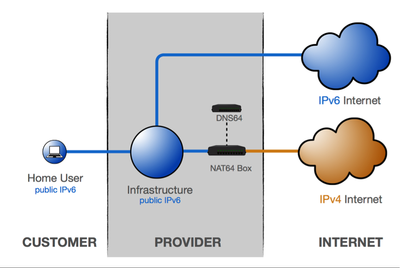
\includegraphics[width=\textwidth,height=\textheight,keepaspectratio]{nat64.png}
\caption{NAT64 visualisatie \autocite{RIPE2016}}
\end{figure}

\section{Besluit}

Bij het gebruiken van deze methodes komt er ook een extra complexiteit bij te pas. Dit zal het netwerk niet vergemakkelijken en hecht een zeker kennis en onderhoud van het netwerk. Deze methodes zouden op elk ogenblik vermeden moeten worden waar mogelijk. Een betere oplossing voor dit probleem zou het toepassen van DS-Lite kunnen zijn. Deze mechaniek heeft een lagere complexiteit en brengt minder nadelen met zich mee.

\chapter{Aftellen van IPv4}
\label{ch:h4}

Dit hoofdstuk bespreekt wat de uitputting van IPv4 juist inhoudt, hoe deze tot zover is kunnen komen en wat een oplossing is om hiermee om te gaan. Ook zal er visueel aangetoond worden hoe we er vandaag de dag tegenover staan en wat er de komende maanden zal gebeuren rond IPv4 uitputting en IPv6.

Op 3 februari 2011 had IANA (Internet Assigned numbers Authority) aangekondigd dat hun vrije IPv4 pool volledig uitgeput was. De IPv4 uitputting betekent niet dat het einde van het internet is aangebroken. Deze term wordt gebruikt om aan te tonen dat er geen niet-toegewezen IPv4 adressen beschikbaar zijn om uit te delen. Door de grote groei aan IoT, mobiele apparaten en andere geconnecteerde apparaten zijn de beschikbare adressen op een zeer snelle en korte tijd uitgedeeld. Dit werd nooit verwacht tijdens de bouw van IPv4 en werd ook niet gemaakt om heel de wereld in contact te brengen met het internet. Als gevolg was er dus het IPv6 protocol ontwikkeld die de uitputting van IPv4 zou wegnemen.

RIPE NCC, die verantwoordelijk is voor Europa, is begonnen op 14 september 2012 met het uitdelen van zijn laatste /8 blok. De /8 blok bevat de laatste beschikbare IPv4 adressen om uit te delen en bevat 16777216 (2 tot de 24) adressen. Volgens de policy van RIPE NCC is het voor de leden enkel mogelijk om een /22 (1024 adressen) blok aan te vragen, ook al kunnen ze grondig aantonen dat er een grotere blok nodig is krijgen ze maar een /22. Ook zal er geen nieuwe PI (Provider Independent) aangesteld worden.

Voor het bereiken van de laatste /8 blok zijn er verschillende fases ondernomen. Fase 0 was het uitdelen van de IPv4 adressen. Op dat moment was er nog geen sprake van een totale uitputting. Tijdens deze fase werden adressen enkel toegewezen als de evaluatie ook volledig afgerond was. Er werden dus ook geen adressen gereserveerd of aan de kant gehouden tijdens deze evaluatie. Verzoeken naar adressen werden grondig gecontroleerd door een IPRA (IP resource Analyst) en voerde interne controle uit \autocite{RIPE2016Fases}.

Het bereiken van fase 1 vond plaats op 4 september 2012. Deze fase werd geactiveerd als er een kritieke toestand plaats vond bij de beschikbare adressen. Op dit moment was er nog een voorraad van één maand of één /10 blok naast /8 om uit te delen. Verder werden de controles zwaarder en grondiger behandeld \autocite{RIPE2016Fases}.

Momenteel situeren we onszelf in fase 2. Deze fase ging van start op 14 september 2012, enkele dagen nadat fase 1 werd bereikt. Bij het begin van deze fase werden alle verzoeken die in de wachtrij stonden bevroren. Zij werden op de hoogte gebracht dat de laatste /8 blok en werd ingezet en verdeeld. Enkel de LIRs die in aamerking komen zullen eenmalig een /22 toegewezen krijgen \autocite{RIPE2016Fases}.

Op 10 april 2018 waren er nog 0.12 miljoen adressen over of 0.01 /8s. Vandaag zijn er geen beschikbare adressen meer over in de blok, dit werd bereikt vanaf 17 april 2018. Nu de laatste blok volledig op is wil dit niet zeggen dat er geen beschikbare adressen meer over zijn. RIPE NCC is momenteel bezig met het herstellen van andere adressen. Deze kunnen gaan van het terugnemen van adressen als een bepaalde LIR is gestopt en van gerecupereerde adressen van IANA’s pool. Maar vooraleer deze adressen worden uitgedeeld en toegewezen blijven ze in quarantaine. Momenteel is er ook geen exacte datum of tijdstip vastgelegd wanneer adressen uit de quarantaine worden gehaald klaar om uitgedeeld te worden  \autocite{RIPE2014}. 

\begin{figure}
\centering
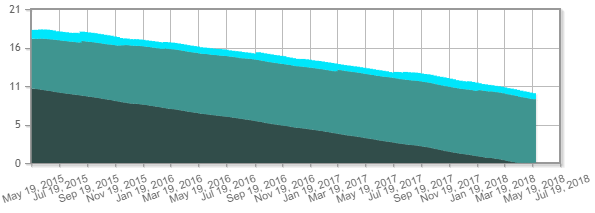
\includegraphics[width=\textwidth,height=\textheight,keepaspectratio]{exhaustion1.PNG}
\caption{IPv4 uitputting \autocite{RIPE2014}}
\end{figure}

Deze grafiek geeft een evolutie aan van beschikbare IPv4 adressen. In bovenstaande grafiek is er duidelijk te zien dat naar gelang de tijd de beschikbare adressen dalen. De donkere kleur staat voor de laatste /8 blok die vrijgegeven is. De licht groene kleur heeft dan meer een stijgende evolutie gekend. Dit zijn de adressen die gerecupereerd zijn van IANA en van LIRs die gestopt zijn. In dit deel komen er dus meer adressen vrij maar blijven ze wel in quarantaine. de blauwe kleur bovenaan toont de gereserveerde adressen aan. Deze worden ingedeeld in een /13 voor tijdelijke toewijzingen, /16 voor IXPs (Internet Exchange Point) en nog een /16 voor onvoorziene omstandigheden die kunnen plaatsvinden. Ook hierin zitten enkele gerecupereerde adressen in quarantaine  \autocite{RIPE2014}.

Op 8 mei 2018 zijn er in totaal nog 9.70 miljoen adressen over waarvan er maar 8.89 miljoen ter beschikking zijn. Zoals we al eerder vernomen hadden, is het aantal in de laatste 185 /8 blok enorm klein. Het aantal beschikbare adressen staat op 0.04 miljoen adressen. Al de gerecupereerde adressen komen samen neer op een 8.85 miljoen adressen. Maar deze zijn dus nog steeds in quarantaine en komen nog niet vrij. De gereserveerde adressen zijn niet beschikbaar en tellen mee voor 0.81 miljoen \autocite{RIPE2014}.

\begin{figure}
\centering
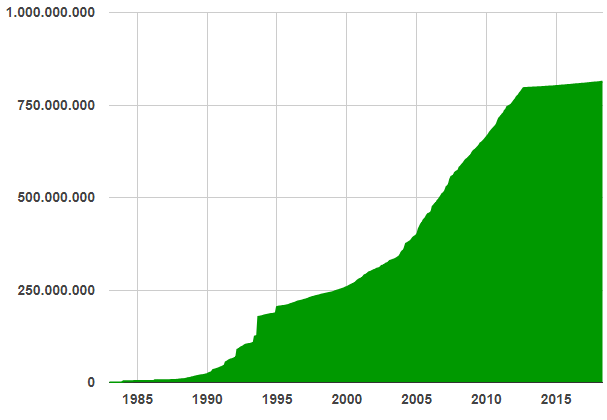
\includegraphics[width=\textwidth,height=\textheight,keepaspectratio]{exhaustion2.PNG}
\caption{IPv4 evolutie \autocite{RIR2018}}
\end{figure}

De grafiek hierboven toont de evolutie van IPv4 in de RIPE NCC zone, ook wel verantwoordelijke voor Europa. De groei dat er is gekomen vanaf de jaren 2000 is immens. Als we verder kijken naar het jaartal 2012, wanneer de laatste 185 /8 blok was aangekondigd, zien we een sterke verandering in de groei. De groei die het tussen het jaar 2012 en heden heeft een zeer kleine stijgingsfactor. Dit komt voornamelijk door de policies die zijn opgesteld door RIPE om met de laatst beschikbare blok voorzichtig overweg te gaan. Hierbij werd er grondig gekeken en in kleinere maten adressen toegewezen waardoor ze zo lang mogelijk de volledige uitputting wilden tegengaan.

\section{Besluit}

Enkele conclusies die er kunnen gemaakt worden zijn, dat komende maanden een hoogtepunt zullen zijn voor zowel IPv4 als voor IPv6. Voor IPv4 kan dit het volledig einde betekenen van de blok wat voor IPv6 een goede zaak kan betekenen. Nu het moeilijker is om nog een range van IPv4 adressen te krijgen gaat er meer overschakelen naar een IPv6 range. Hierdoor zal de vraag naar IPv6 stijgen en de ontwikkeling en overgang sneller in gang gezet worden.  

\chapter{IPv6 op globaal niveau}
\label{ch:h5}

In dit hoofdstuk zal er dieper worden ingegaan op de adoptie van IPv6 op verschillende niveaus. Er zal bekeken worden hoe deze overgang loopt op zowel globaal niveau als een klein deel op Europees en Belgisch niveau. Dit zou een goede schets moeten geven over hoe het er in België momenteel aan toe gaat en of we al dan niet een betere verhouding hebben dan andere landen. 

\section{Hoe staat IPv6 er tegenover}

Het is ook al eerder geweten dan vandaag dat de uitputting van IPv4 tot zijn einde is gekomen. De beschikbare adressen zijn bijna volledig uitgedeeld en het einde is nabij. Als gevolg hiervan was er IPv6 ontwikkeld om IPv4 over te nemen na zijn uitputting. Dankzij de ‘World IPv6 Day’ is de groei en het aantal gebruikers van IPv6 zeker gestegen. Vanaf deze dag is IPv6 officieel aangekondigd als opvolger van IPv4. 

\section{IPv6 op globaal niveau}

IPv6 is wereldwijd bekend, het nieuwe internet protocol. Hier zal er verder onderzocht worden wat de huidige status is over het internationale gebruik van IPv6. Hoe bedrijven, landen en gebruikers zich hieraan gaan aanpassen en of dit wel effectief bekend is en gebruikt wordt. Het globaal bekijken van het gebruik van IPv6 kan op verschillende manieren gebeuren. Er zal gebruik gemaakt worden van grafieken die geanalyseerde data grafisch zal voorstellen. Verschillende grafieken zullen vergelijkingen weergeven op verschillende aspecten die onderzocht kunnen worden. Alsook het analyseren van globale enquêtes. 

Een eerste grafiek zal aantonen hoeveel gebruikers er zijn, die Google bereiken over IPv6. Deze grafiek geeft een duidelijke weergave van de groei die afgelopen jaren volgde en vooral vanaf 2011, de dag waarop IPv6, begon met evolueren. De laatste meting was op 22 mei 2018 en bevatte een totaal van 19.25\% IPv6 gebruikers. Dit wilt verder zeggen dat bijna 1 op de 5 personen Google bereikt via IPv6. 

\begin{figure}
\centering
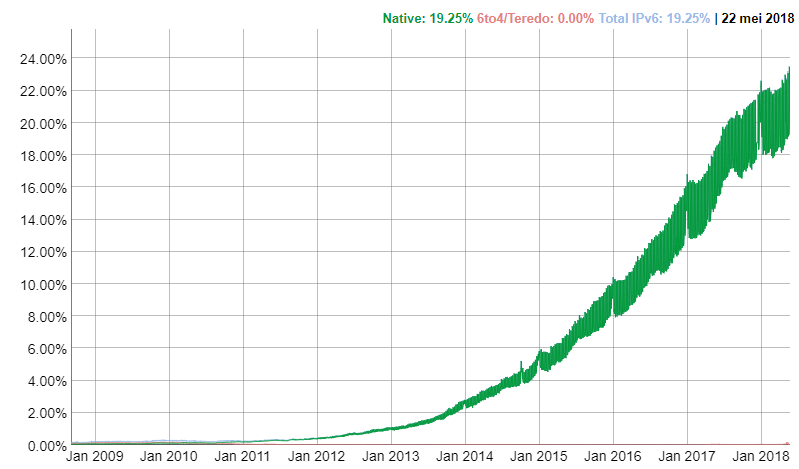
\includegraphics[width=\textwidth,height=\textheight,keepaspectratio]{googleIPv6.png}
\caption{IPv6 evolutie van Google \autocite{GoogleIPv6}}
\end{figure}

Een volgende grafiek geeft weer hoeveel /48 blokken er uitgedeeld zijn van IPv6. Als we deze grafiek dieper gaan onderzoeken, zijn er twee stijgingen te zien. De eerste stijging vond plaats vanaf 2004 tot en met 2006. Deze evolutie is vooral te danken aan de eerste opkomst van IPv6. De tweede groei, waarbij deze nog niet is gestopt en dus nog steeds aan het doorgroeien is, is begonnen in 2011. Hier kunnen we zeggen dat dit gekomen is door de dag van IPv6 dat was uitgeroepen in 2011. Ook is er te zien dat vanaf het jaar 2011 een blijvende stijging is wat het zeer goed maakt voor de populatiegroei van IPv6. De laatste meting, op 1 mei 2018, telt 15.281.735.778 /48 blokken wereldwijd. 

\begin{figure}
\centering
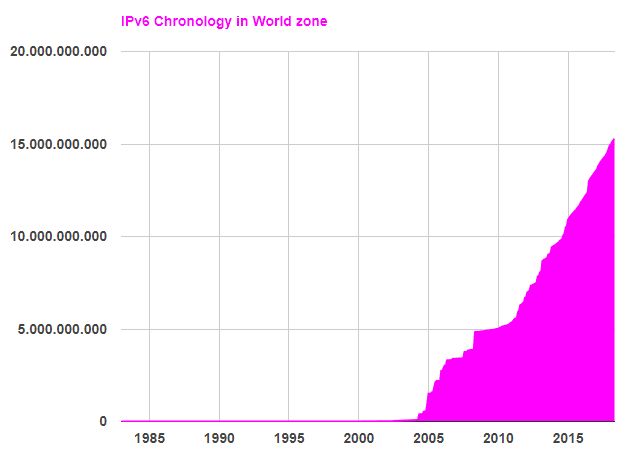
\includegraphics[width=\textwidth,height=\textheight,keepaspectratio]{48blokIPv6.PNG}
\caption{IPv6 /48 blok visueel \autocite{RIR2018}}
\end{figure}

Onderstaande grafiek geeft ons een breder beeld over het percentage netwerken, autonome systemen, dat een IPv6 prefix aankondigd. Globaal gezien is er een gemiddelde van 24.37\%, waarvan 14738 van de 60473 Ases, IPv6 geactiveerde netwerken. Deze laatste meting werd genomen op 1 maart 2018.

\begin{figure}
\centering
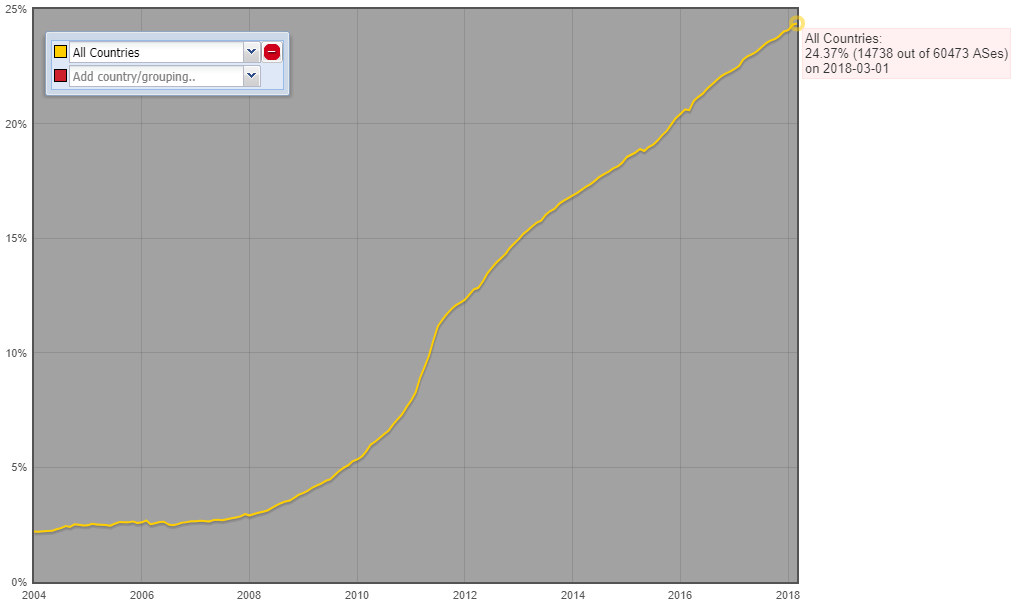
\includegraphics[width=\textwidth,height=\textheight,keepaspectratio]{asIPv6.PNG}
\caption{IPv6 autonome systemen \autocite{RIPE2016}}
\end{figure}

Er is ook een duidelijk overzicht van welk land het beste scoort op verschillende onderdelen van IPv6 gebruik. Dit gebruik kan onderverdeeld worden in 4 verschillende categorieën namelijk, Web, Email, DNS en IPv6 actieve gebruikers.

Vervolgens heeft RIPE enkele enquêtes opgesteld om te meten wat de ondervindingen zijn en hoe het zit met het uitrollen van IPv6. Hiermee kan er onderzocht worden hoe de aanpak, adoptie en aanvaardingen zijn van IPv6. Verder gaan er enkele enquêtes aangekaart worden en met elkaar vergeleken worden. Deze zullen een duidelijk overzicht geven van de overgang van IPv6 op jaarniveau. Hiermee kan er onderzocht worden hoe groot de evolutie is op de voorbije jaren.

De eerste enquête die werd opgesteld dateert van 14 November 2016, de intentie hiermee was om een breder beeld te creëren over de huidige uitrolling van IPv6 was, specifiek gericht op ISP’s. 

De eerste grafiek geeft een zeer informatief beeld terug. Hierop is beter te zien dat de respons op de enquête uit twee soorten gebruikers bestaat. De eerste groep heeft IPv4 gebruikt, de andere groep gebruikte IPv6 om deze enquête te beantwoorden. Dit geeft ons dus al een beter beeld van hoeveel percent van de gebruikers het IPv6 protocol hanteren. In 2016 was dit maar liefst 31\%, 372 van de 1199 deelnemers, hebben over IPv6 beantwoord. 

\begin{figure}
\centering
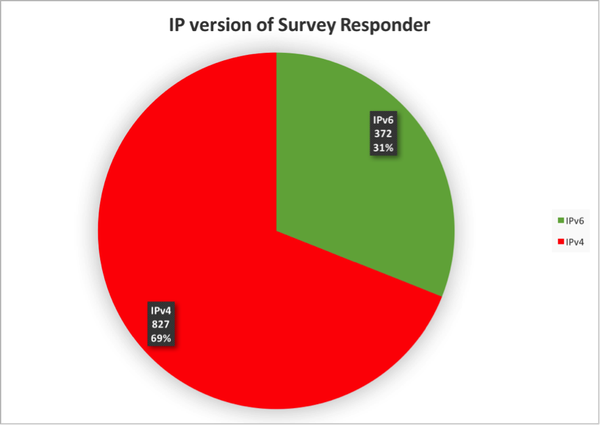
\includegraphics[width=\textwidth,height=\textheight,keepaspectratio]{survey2016_aantal.png}
\caption{IPv6 survey 2016 respons \autocite{Martinez2016}}
\end{figure}

Een volgende grafiek geeft beter aan van waar deze deelnemers komen en onder welke instantie ze vallen. Met instanties wordt er bedoeld onder welke regio de deelnemers vallen. Op onderstaande grafiek is er dus duidelijk te zien dat de meeste uit de regio RIPE NCC komen. Deze instantie is verantwoordelijk voor de Europese kant. Waaronder ARIN verantwoordelijke is voor de Amerikaanse regio, AfriNIC voor de Afrikaanse, APNIC voor de Aziatische en de LACNIC voor de Latijns-Amerikaanse regio.

\begin{figure}
\centering
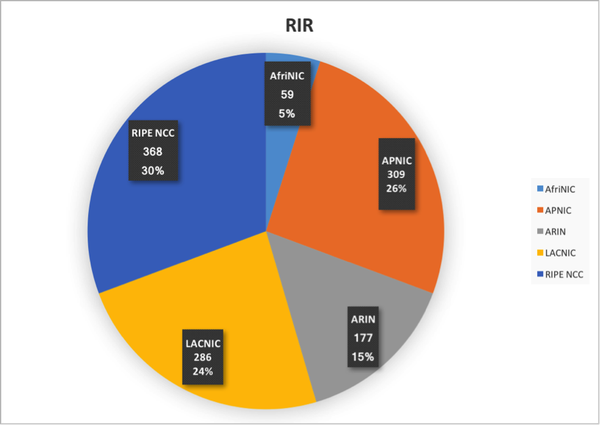
\includegraphics[width=\textwidth,height=\textheight,keepaspectratio]{survey2016_rir.png}
\caption{IPv6 survey 2016 RIR \autocite{Martinez2016}}
\end{figure}

Hoe gecommercialiseerd is IPv6 binnen de ISP’s nu? Wel, volgende grafiek geeft hierop een duidelijker beeld. Er wordt aangetoond dat 31\% van de ISP’s gebruik maken van IPv6 en commercieel actief mee bezig zijn. 17\% van de ISP’s is nog niet actief en dus ook nog niet commercieel actief, of zit momenteel in de test fase voor verdere stappen te ondernemen. De overige 52\% heeft deze vraag niet beantwoord. Daardoor kunnen we besluiten dat van alle deelnemers er 64\% van de ISP’s actief bezig is.

\begin{figure}
\centering
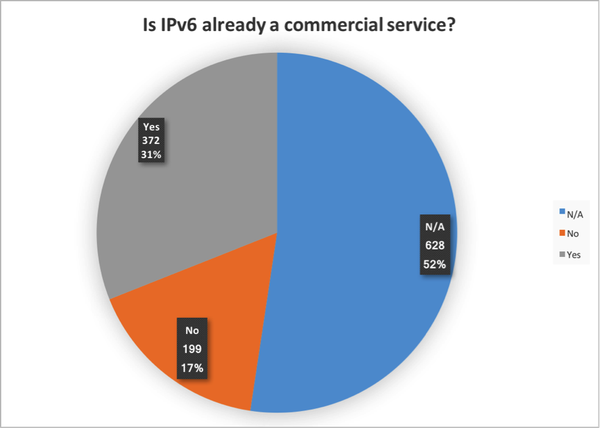
\includegraphics[width=\textwidth,height=\textheight,keepaspectratio]{survey2016_actief.png}
\caption{IPv6 survey 2016 commercieel \autocite{Martinez2016}}
\end{figure}

Op vlak van technologie is er veel keuze om klanten gebruik te laten maken van IPv6. Om een beter beeld te geven van de geprefereerde technologie keuzes van ISP’s is hieronder een grafiek die deze vraag beantwoord. Op het eerste zicht is er een groot deel dat gebruik maakt van FTTH, 35\%, xDSL, 22\%, en via kabel of DOCSIS, 20\%. 

\begin{figure}
\centering
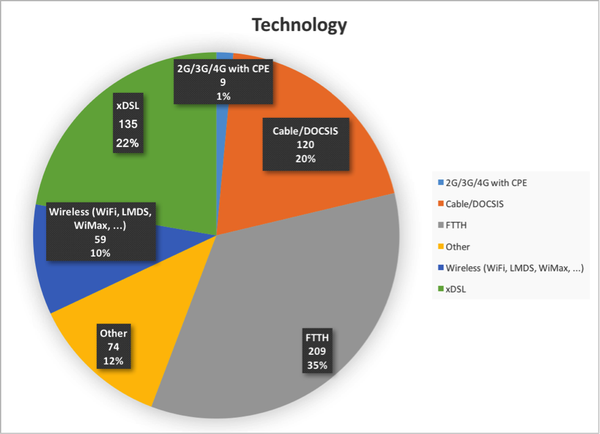
\includegraphics[width=\textwidth,height=\textheight,keepaspectratio]{survey2016_technologie.png}
\caption{IPv6 survey 2016 technologie \autocite{Martinez2016}}
\end{figure}

De laatste grafiek zal een verduidelijking weergeven op de gebruikte transitie mechanismen van een ISP. Bij transitie mechanisme zijn er veel verschillende methodes, maar welke het meest gebruikt worden onder de ISP’s is belangrijk om te weten. Op onderstaande grafiek is er een duidelijke winnaar. De methode die het meeste gehanteerd wordt is Dual-stack met een publiek IPv4 en Global unicast adres, GUA. In hoofdstuk 3 werd er dieper ingegaan op enkele methodes en uit de conclusie blijkt dat er een voorkeur was naar Dual-stack, wat hier ook bewezen is.

\begin{figure}
\centering
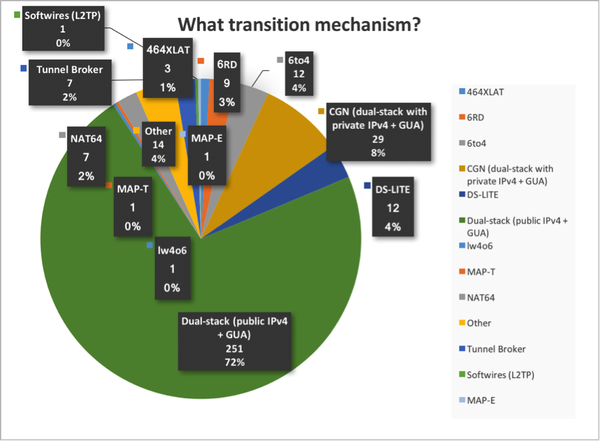
\includegraphics[width=\textwidth,height=\textheight,keepaspectratio]{survey2016_transitie.png}
\caption{IPv6 survey 2016 transitie \autocite{Martinez2016}}
\end{figure}

Om de evolutie op een jaar tijd te bekijken, gaan we deze resultaten vergelijken met de enquête die dateert van 13 oktober 2017. Met deze update is er een beter zicht mogelijk op de evolutie van IPv6 op een jaar tijd. Hierbij zullen de uitslagen vergeleken worden met de enquête van 2016. 

Opnieuw werd er gekeken hoever de commercialisatie stond van IPv6 bij ISP’s. Bij het opnieuw stellen van deze vraag is er een duidelijk verschil van resultaten ten opzichte van het vorige jaar.  Het grootste verschil is het aantal deelnemers die deze vraag niet beantwoord hadden. Bij de laatste update werd deze vraag volledig beantwoord en gaf dit een beter beeld van de effectieve commerciële diensten. Er waren maar liefst voor 65\%, 438 van de 673 deelnemers, van de antwoorden een ja-stem. Dit wil zeggen dat 65\% van de deelnemers actief bezig is met het aanbieden van IPv6 aan klanten. Waaronder het jaar ervoor maar 199 ISP’s bezig waren met het verdelen van IPv6.

\begin{figure}
\centering
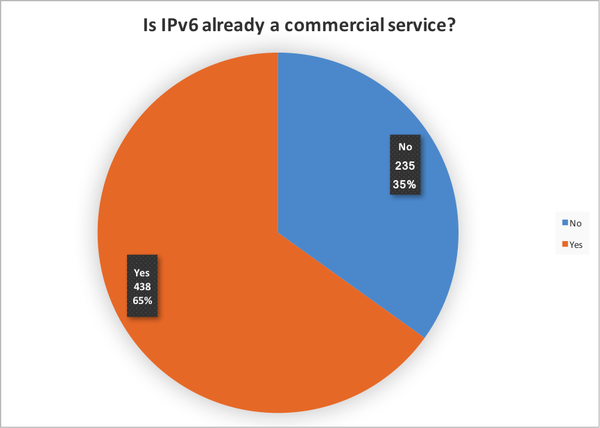
\includegraphics[width=\textwidth,height=\textheight,keepaspectratio]{survey2017_actief.png}
\caption{IPv6 survey 2017 commercieel \autocite{Martinez2017}}
\end{figure}

Op vlak van de gebruikte technologieën zijn er weinig veranderingen gebeurt op jaarbasis. De meest gehanteerde methodes blijven FTTH, xDSL en 3G broadband als bijkomende methode. Deze zijn voorlopig de meeste populaire technologieën. Hoewel in het jaar 2016 DOCSIS populair was, is deze verminderd naar gebruik toe.

Ook is er een overgang van gebruikte transitie mechanieken. Hierdoor blijkt dat nieuwere en recentere methodes worden gehanteerd in plaats van de oudere technieken. Het is zo dat er een groei is in het gebruik van 464XLAT en dual-stack met publieke IPv4 adressen. Verder is het zeker belangrijk om een nieuw evolutie-onderzoek op te stellen van het jaar 2017 tot 2018. Dit zou een nog beter zicht moeten geven over wat er echt aan het doorgroeien is naar een standaardoplossing voor dergelijke methodieken om met IPv6 te werken.

In 2018 werd er een interessante update van een bepaalde enquête uitgevoerd. Deze ging eerder over de adoptie wereldwijd en niet zozeer gefocust op ISP’s. Deze enquête werd uitgevoerd in verschillende jaren zoals 2008, 2009, 2011, 2012 en het laatste jaar 2013. Nu in 2018 werd er een update gemaakt voor de evolutie om de afgelopen 5 jaar te weerspiegelen en opnieuw informatie te verzamelen. RIPE heeft deze uitgevoerd en de eerste resultaten werden voorgesteld op het RIPE76 evenement in Marseille op 14-18 mei 2018. De uitgebreide resultaten zullen worden voorgesteld op 6 juni op het Educa evenement. Daarom zullen de eerste resultaten al onderzocht worden in deze scriptie.

In de verkregen resultaten is er te zien dat er ongeveer een 50\% van de antwoorden vooral uit grote ISP’s is gekomen, voor 30\% aan educatieve instellingen en ICT instellingen en voor 20\% aan overheid, onderzoekers en andere instellingen. Deze indelingen komen overeen met de jaren ervoor wat het zeer goed maakt omdat het over dezelfde aantal soorten instellingen gaat. Het probleem bij deze enquête was dat deze niet bereikbaar zijn vanaf IPv6. Waardoor er enkele resultaten wegvielen maar volgens RIPE was dit de bedoeling omdat deze hetzelfde moest opgesteld zijn als de jaren er voorheen.

Opvallende data die was geanalyseerd was de IPv6 allocatie. IPv6 allocatie betekent het toewijzen van adresruimte naar IR (Internet Registry) om op hun beurt terug die adresruimte door te verdelen. Momenteel staat het op 85\% IPv6 allocatie. Dit komt neer op een groei van 20\% met het jaar 2012 en een groei van 10\% met 2013. Het is logisch dat deze momenteel minder en minder zal groeien. Het is dus nog niet de bedoeling om 100\% al toe te wijzen en te verdelen.

\begin{figure}
\centering
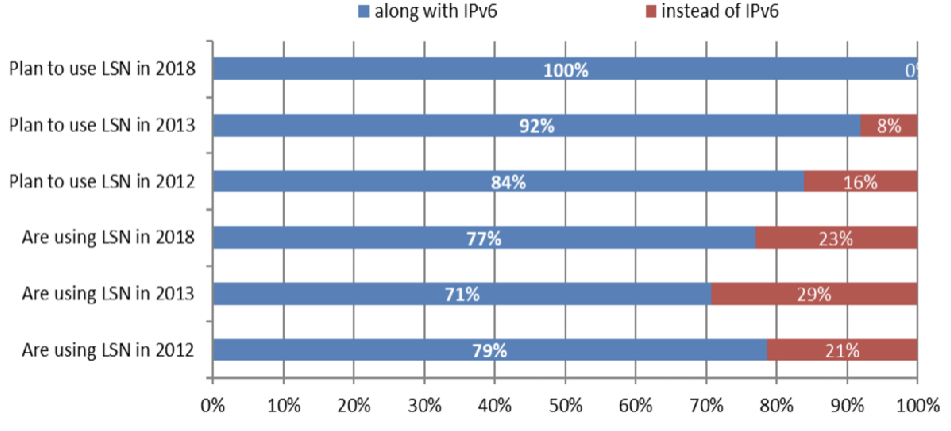
\includegraphics[width=\textwidth,height=\textheight,keepaspectratio]{survey2018_cgn.PNG}
\caption{IPv6 survey 2018 CGN/LSN \autocite{Massimiliano2018}}
\end{figure}

Alweer zijn de transitie technieken onderzocht en geanalyseerd naar welke het meeste aanvaard en gebruikt worden. Volgens deze data gebruikt meer dan 50\% geen transitie methode. Van diegene die wel deze technologie gebruiken kan er het volgende worden afgeleid. Op deze grafiek is er duidelijk te zien dat NAT64 een groot deel in beslag neemt en de populairste methode is. Daarnaast hebben DS-Lite en 6RD ook hun gebruikers maar bevatten deze een kleinere populariteit.

\begin{figure}
\centering
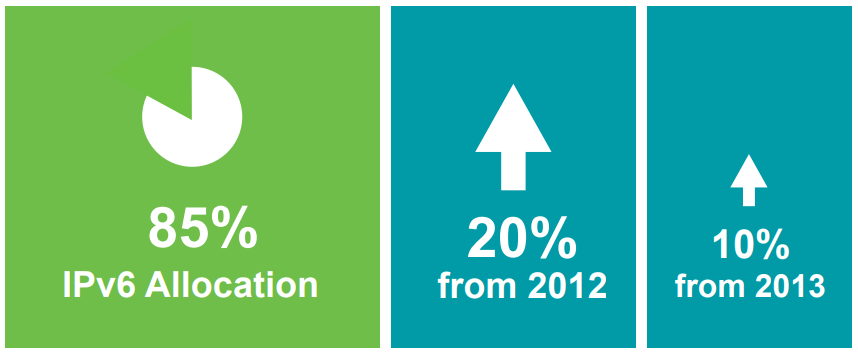
\includegraphics[width=\textwidth,height=\textheight,keepaspectratio]{survey2018_allocatie}
\caption{IPv6 survey 2018 verdeling \autocite{Massimiliano2018}}
\end{figure}

Ook is er iets interessant uitgehaald uit de verkregen data. Het gebruik maken van CGN (Carrier Grade NAT) of LSN (Large Scale NAT) samen of in plaats van IPv6. Met deze grafiek is er een zeer goed zicht op de toekomst van IPv6. In het jaar 2012 was er 16\% dat koos om deze technologie, CGN/LSN, te gebruiken in de plaats van IPv6. Het jaar daarop was dit met de helft verminderd en momenteel in 2018 staat het aantal geplande op 0\%. Dit is goed omdat men op deze manier gaat samenwerken met het IPv6 protocol en niet proberen deze te vervangen. Momenteel gebruiken er wel nog 23\% van deelnemers CGN/LSN als vervanger van IPv6. Als we dit vergelijken met het jaar 2013 zien we een kleine daling wat het overschakelen van vervangen naar samen met verbeterd. De komende jaren mogen we dus zeker verwachten dat deze enkel maar gaat afnemen omdat de geplande vervanging 0\% bevat.

\begin{figure}
\centering
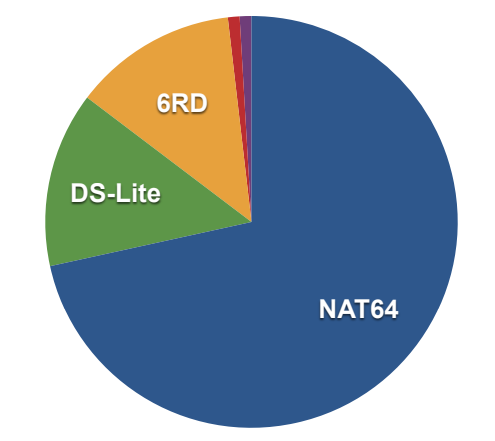
\includegraphics[width=\textwidth,height=\textheight,keepaspectratio]{survey2018_transitie.PNG}
\caption{IPv6 survey 2018 transitie \autocite{Massimiliano2018}}
\end{figure}

Nu we weten hoe het al gaat met IPv6, blijven er toch velen achter en durven ze vaak de stap niet te zetten naar IPv6. Daarom was er een bepaalde vraag gesteld om te achterhalen waarom het ondersteunen van IPv6 niet direct gebruikt wordt. Hier kwam er als duidelijk antwoord dat de kennis, bijkomende kosten en het overbrengen naar niet technische afdelingen het moeilijk maakt om dit te volbrengen. Als deze antwoorden werden vergeleken met de jaren voordien dan ziet men dezelfde antwoorden steeds terugkomen. Daarom blijft er vaak de vraag waarom er nog steeds geen verandering volgde en wat men daaraan kan doen.

In het volgende hoofdstuk zal er vooral dieper ingegaan worden op de adoptie in België en hoe deze daar aan het evolueren is. Aan de hand van grafieken zal er een duidelijk overzicht gegeven worden over de huidige aanpak van IPv6 op de Belgische markt.





\chapter{Belgische bedrijven en IPv6}
\label{ch:h6}

\section{IPv6 Adoptie}

Op onderstaande afbeelding van Google is er te zien dat België momenteel een IPv6 adoptie heeft van 52.22\%. Dit wil zeggen dat 52.22\% van de gebruikers IPv6 connectie gebruikt om over Google te surfen. Dus meer dan de helft van het verkeer gaat over IPv6. Volgens de statistieken van Google is België het hoogste land met zoveel IPv6 connectiviteit. Hoe groener het land, hoe groter de adoptie. Terwijl het wereldwijde aantal maar 20.74\% bevat. Dan heeft België meer dan het dubbele aantal dan het wereldwijde gebruik. Dit maakt België het land met het hoogste aantal IPv6 gebruikers van de wereld.

\begin{figure}
\centering
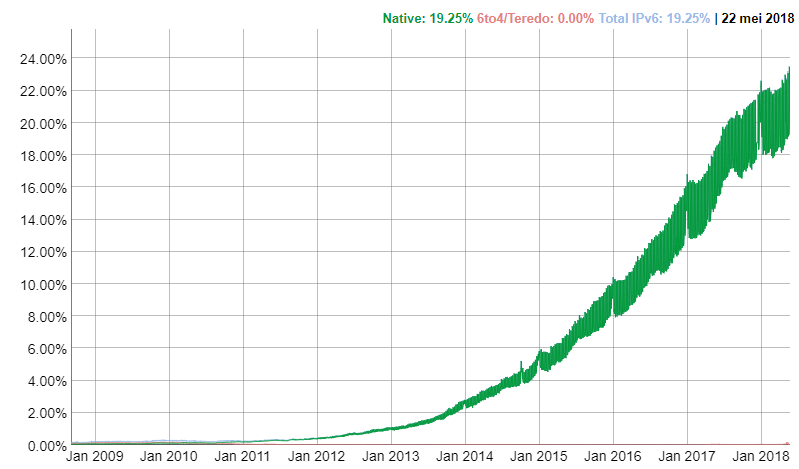
\includegraphics[width=\textwidth,height=\textheight,keepaspectratio]{googleIPv6.png}
\caption{IPv6 status IPv6 in België \autocite{GoogleIPv6Belgie}}
\end{figure}

Nog belangrijk om na te gaan zijn de webbrowsers die IPv6 bereikbaar maken. Dit is een zeer belangrijk element en zeker voor de Belgische bedrijven. Omdat meer en meer gebruik wordt gemaakt van IPv6 en er vaak nog alleen IPv6 gebruikt wordt, is het belangrijk dat bedrijven zich hieraan gaan aanpassen. Als een website van een webshop enkel via IPv4 bereikbaar is dan kunnen de IPv6 klanten geen online shoppingen doen bij deze winkel. Hiervoor is het belangrijk dat bedrijven er zich van bewust zijn dat de webbrowsers zowel IPv4 als IPv6 toegankelijk moeten maken. In onderstaande grafiek is er te zien wat de status is van IPv6 toegankelijke webbrowsers en hoe de evolutie hiervan in de toekomst geschat kan worden. Om de evolutie hiervan te berekenen is er gebruik gemaakt van een logistische s-curve en een voorspelling op de komende 4 jaar of 1460 dagen. Op 26 mei waren er 52.27\% van de sites IPv6 toegankelijk. Volgens de berekeningen zal de 90\% behaald worden op 9 mei 2019, of minder dan 1 jaar zou er 90\% van de Belgische webbrowsers IPv6 actief moeten zijn.

\begin{figure}
\centering
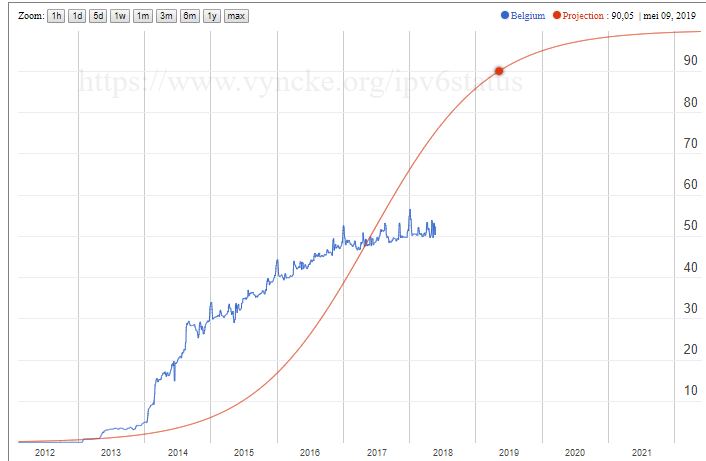
\includegraphics[width=\textwidth,height=\textheight,keepaspectratio]{IPv6vervolg.png}
\caption{IPv6 vervolg op 4 jaar \autocite{Vyncke2018}}
\end{figure}

Het is alvast zeker dat België het beste presteert op het aantal gebruikers over IPv6. Nu rest er enkel nog de vraag waarom België meer gebruikers heeft dan eender welk land. Voor deze vraag heeft Eric Vyncke, mede-eigenaar van de Belgische IPv6 Council, een mogelijk antwoord. Het biedt enkele mogelijkheden die een rol kunnen spelen waarom België zo’n hoog percentage behaald. De eerste mogelijkheid is er omdat België een vrij klein land is en dicht bevolkt. Omdat het land vrij klein is, is de afstand dus ook klein. Daarom wordt er ook vaak gebruik gemaakt van kabel of xDSL aansluitingen. Ook omdat veel van de Belgische ISP’s een tekort hadden aan IPv4 adressen, was er snel een oplossing door gebruik te maken van IPv6. Ook is er een soort van geheim tussen de verschillende ISP’s, cyberpolitie, regelgevers en de minister van economische zaken om het delen van 1 IPv4 adres maximum te beperken tot 16 abonnees. Dit had een grote invloed op het gebruik van NAT/CGN. Als de cultuur van België nader wordt bekeken dan is het een mix van zowel een Duitse als Latijnse cultuur. Dit wil ook zeggen dat er vaak gekeken wordt op een langere termijn en dat er niet veel wordt aangetrokken rond de processen. Ook hebben de drie grote ISP’s van België samengezeten om het gebruik van IPv6 te verduidelijken. Hierbij hebben ze vooral ervaring en een routekaart  met elkaar gedeeld om de evolutie te vergemakkelijken. Dit zijn enkele redenen volgens Eric Vyncke, waarbij hijzelf zegt dat er geen duidelijke reden hiervoor is en dit enkel maar veronderstellingen zijn.

\section{Enquête aan Belgische bedrijven}

Voor een breder beeld te krijgen over hoe het er in sommige bedrijven aan toe zijn, is er een enquête opgestuurd naar verschillende experten. De enquête en opgestelde vragen kan u terugvinden in de bijlagen om de corpus van de scriptie te bewaren. Deze vragen zijn vooral gericht op hoe het bedrijf er tegenover staat, IPv6. Het intern netwerk draaiende op IPv4, IPv6 of beiden. Hoe het zit met de kennis over IPv6, advies geven hiervan, begrippen herkennen en meer. Om de resultaten samen te vatten is er te merken dat er nog geen geval is van een IPv6 only intern netwerk. Zowel IPv4 als een IPv4/IPv6 structuur is al te vinden in een intern netwerk van bedrijven. Als er dan eerder de vraag werd gesteld of er toekomst plannen waren voor een mogelijke implementatie dan kwam er ook de respons dat ze er nog niet mee bezig waren en nog niet aan dachten om dit te implementeren in hun netwerk. Met de vraag of ze zouden kiezen voor een IPv4/IPv6 of een IPv6 structuur, dan kwam er een duidelijk antwoord dat ze allemaal voor gemengd kozen. Dit omdat men de overgang in een langzame beweging zouden volbrengen en omdat IPv4 nog steeds populair blijft. Alsook omdat niet al het apparatuur IPv6 compatibel is in vele gevallen. Er werd ook een bedrijf ondervraagd dat niet hoofdzakelijk met ICT diensten bezig is maar wel hun eigen afdeling heeft. Zij zouden voor deze overschakeling grotendeels gebruik maken van hun interne werkkracht maar zouden toch nog extra externe expertise raadplegen terwijl bij een IT consultancy bedrijf genoeg interne werkkracht heeft met de kennis van IPv6. Als er werd nagegaan over de kennis van IPv6, door het ondervragen van een begrip namelijk SLAAC, dan had niemand daar een probleem mee deze ook te beantwoorden. Wat wil leiden tot een beginkennis van IPv6. De voornaamste redenen om de overschakeling nog niet te beginnen is vooral door de complexiteit van de overgang en kennis van de engineers. Maar ook omdat sommige infrastructuren er nog niet klaar voor of nog niet compatibel hiermee zijn. Wat ook een reden was dat klanten geen nieuwe investeringen willen doen in de ICT infrastructuur en zeker nog niet met de start van GDPR (General Data Protection Regulation). Als ze zichzelf een score op 5 moeten geven dan scoort deze maximaal 2.5/5 voor kennis in IPv6. Dit toont nogmaals aan dat er te weinig opleidingen en opvolging is van het nieuwe internet protocol. Hierin zal in de toekomst meer geïnvesteerd moeten worden als men hiermee meer te maken zal hebben. Ook is er gevraagd geweest naar de toegankelijkheid van hun webbrowsers. We hebben zowel het antwoord ja als nee gekregen. Dit toont erop aan dat men toch rekening aan het houden is met de toegankelijkheid van hun sites. Ook bij degenen waarbij ze nog niet IPv6 actief zijn, blijft het antwoord dat het momenteel nog niet zo is, wat wil duiden op toekomstige plannen. De laatste vraag die besproken zal worden gaat over hoe ze in aanraking gekomen zijn met IPv6. We zien hierbij vooral dat er toch al trainingen en seminaries worden gevolgd. Alsook het behalen van certificaten en in contact komen met partners en datacenters. Ook bij de twee grootste Belgische IPS’s, Telenet en Proximus, is het mogelijk om als klant gebruikt te maken van IPv6. Als men thuis een IPv6 verbinding wilt hebben dan bieden ze beiden ook een zeer goede ondersteuning hiervoor aan.

Een besluit die we hieruit kunnen trekken is dat er toch al bedrijven actief met IPv6 aan het werken zijn maar eerder gedeeld met IPv4. Dit maakt het ook beter om al een ruimere kennis op te doen. Ook is eruit af te leiden dat de kennis totaal nog niet op een hoog punt staat, maar dat er gezegd kan worden dat er trainingen gevolgd worden. 


%%=============================================================================
%% Conclusie
%%=============================================================================

\chapter{Conclusie}
\label{ch:conclusie}

%% TODO: Trek een duidelijke conclusie, in de vorm van een antwoord op de
%% onderzoeksvra(a)g(en). Wat was jouw bijdrage aan het onderzoeksdomein en
%% hoe biedt dit meerwaarde aan het vakgebied/doelgroep? Reflecteer kritisch
%% over het resultaat. Had je deze uitkomst verwacht? Zijn er zaken die nog
%% niet duidelijk zijn? Heeft het onderzoek geleid tot nieuwe vragen die
%% uitnodigen tot verder onderzoek?

%%\lipsum[76-80]

De conclusie die uit deze scriptie kan gehaald worden is dat men zowel op globaal als op Belgische vlak zeer sterk bezig is met de adoptie van IPv6. De meeste bedrijven, vooral ISP’s, zijn er zich van bewust dat het werken met IPv6 een vereiste zal worden. Ook de afgelopen jaren was er een toenemende groei van het gebruik hiervan en zal de komende maanden en jaren alleen maar verbeteren. Hiervoor is het ook zeker belangrijk om de groei op een jaarlijkse basis goed bij te houden zodanig men dit als motivatie voor bedrijven kan gebruiken. Ook is België het beste land met het aantal gebruikers die IPv6 hanteren wat een totale verrassing is voor vele Belgen.

Alsook biedt deze scriptie enkele antwoorden op de onderzoeksvragen. Er is een duidelijk overzicht van hoe de adoptie en aanvaarding van IPv6 staat op globaal niveau. Volgens Google stond deze op 23.33\% op 26 mei 2018. Wat het toch al meer dan 1/5 van al het verkeer maakt. Na 7 jaar sinds de eerste IPv6 wereld dag kan men dit zeker niet slecht noemen. Als er nog een duidelijker zicht wilt gegeven worden is het nodig om per land zijn evolutie te gaan bekijken.

Om enkele antwoorden te bieden op de onderzoeksvragen omtrent de evolutie op Belgisch niveau, dan kunnen we zeggen dat België het beter doet dan verwacht. Zoals eerder vernoemd, scoort België het beste op vlak van IPv6 gebruikers over heel de wereld wat het zeer interessant maakt. Om hierover een duidelijke verklaring te geven is moeilijk maar de gegeven veronderstellingen van Eric Vyncke kunnen hier zeker een invloed op hebben. Er kan ook afgeleid worden uit de enquêtes dat er toch al aan IPv6 gedacht wordt en dat hiermee al effectief in een werkomgeving mee geëxperimenteerd wordt. Alsook kan er geconcludeerd worden dat er nog veel groeipotentieel is naargelang het gebruik maken van IPv6 en dan niet zo gericht op de implementatie. Enkele hoofdredenen waarom bij de meeste bedrijven nog niet een implementatie is doorgekomen is vooral het gebrek aan kennis van het protocol. De noodzaak is dat bedrijven extra investeringen moeten doen omtrent trainingen, cursussen, certificatie en seminaries. Er kan ook gezegd worden dat de overgang van IPv4 naar IPv6 niet op één dag kan gebeuren maar dat dit vooral veel tijd, werk en planning in beslag neemt. Er wordt dus ook een IPv4/IPv6 verkozen in plaats van een IPv6 only netwerk. Wat vooral te maken kan hebben met de comptabiliteit van de apparaten in de infrastuur als met de kennis die engineers momenteel hebben over het protocol.

Er wacht IPv6 een veelbelovende toekomst te wachten waaraan bedrijven zich meer en meer bewust van beginnen te worden dat het hoe dan ook een vereiste is om hiermee in aanraking te komen. 


%%=============================================================================
%% Bijlagen
%%=============================================================================

\appendix

%%---------- Onderzoeksvoorstel -----------------------------------------------

\chapter{Onderzoeksvoorstel}

Het onderwerp van deze bachelorproef is gebaseerd op een onderzoeksvoorstel dat vooraf werd beoordeeld door de promotor. Dat voorstel is opgenomen in deze bijlage.

% Verwijzing naar het bestand met de inhoud van het onderzoeksvoorstel
%---------- Inleiding ---------------------------------------------------------

\section{Introductie} % The \section*{} command stops section numbering
\label{sec:introductie}

Mijn onderzoek zal gaan naar hoe de overschakeling binnen bedrijven van IPv4 (Internet Protocol version 4) naar IPv6 (Internet Protocol version 6) verloopt. Zijn de bedrijven in hun netwerk bezig naar het overschakelen naar het vernieuwde internet protocol, die noodzakelijk was binnen het internet, of ze het van plan of hebben ze er helemaal nog niet bij stilgestaan. Om dit onderzoek tot een succes uit te voeren, zal ik gebruik maken van een enquête en de antwoorden doorgronden of deze al dan niet terechte opmerkingen zijn.

%---------- Stand van zaken ---------------------------------------------------

\section{State-of-the-art}
\label{sec:state-of-the-art}

Deze scriptie zal gaan over de huidige stand van zaken van de adoptie van IPv6 op zowel globaal niveau als op Belgisch niveau. Er zal een studie uitgevoerd worden en enquêtes onderzocht worden. Dit dient ervoor om het standpunt van een bedrijf naar boven te brengen en de verkregen resultaten te doorgronden. 

% Voor literatuurverwijzingen zijn er twee belangrijke commando's:
% \autocite{KEY} => (Auteur, jaartal) Gebruik dit als de naam van de auteur
%   geen onderdeel is van de zin.
% \textcite{KEY} => Auteur (jaartal)  Gebruik dit als de auteursnaam wel een
%   functie heeft in de zin (bv. ``Uit onderzoek door Doll & Hill (1954) bleek
%   ...'')


%---------- Methodologie ------------------------------------------------------
\section{Methodologie}
\label{sec:methodologie}

Om mijn onderzoek uit te voeren zal ik gebruik maken van vragenlijsten. Hierdoor zullen mijn onderzoeksvragen beantwoord worden en is er een duidelijk overzicht over het gebeuren binnen een netwerk van een bedrijf. Aan de hand van deze antwoorden kan er gekeken worden of deze al dan niet doorgrond zijn en of deze terechte antwoorden zijn. Ook zullen er veel data van enquêtes overlopen worden en geanalyseerd. Deze zullen steeds grafisch voorgesteld worden in grafieken. 

%---------- Verwachte resultaten ----------------------------------------------
\section{Verwachte resultaten}
\label{sec:verwachte_resultaten}

De verwachte resultaten zijn dat men ziet dat enkele bedrijven al rekening houden met de overstapping naar het vernieuwde internet protocol IPv6. Ook zal het aantal niet immens groot zijn en zeker onder de helft van het aantal ondervragen bedrijven zitten. Alsook dat nog niemand de grootste stap richting de overgang heeft gemaakt en zeker niet volledig het IPv6 protocol zal hanteren maar eerder samen met IPv4.

%---------- Verwachte conclusies ----------------------------------------------
\section{Verwachte conclusies}
\label{sec:verwachte_conclusies}

Mijn verwachtingen zijn dus dat er van geen enkel van de ondervraagde bedrijven een bedrijf is waarin ze volledig IPv6 zullen hanteren. Ik vermoed ook dat uit het onderzoek zal blijken dat er toch enkele bedrijven er zich van bewust zijn en toch de stap aan het maken zijn voor eerder een gemengde oplossing te gebruiken, dus IPv4 en IPv6 samen. Maar het grootste deel zal zeker nog niet in de richting gaan van een mogelijke implementatie van het protocol.



%%---------- Andere bijlagen --------------------------------------------------
% TODO: Voeg hier eventuele andere bijlagen toe
%\input{...}

%%---------- Referentielijst --------------------------------------------------

\printbibliography[heading=bibintoc]
%\addcontentsline{toc}{chapter}{\textcolor{maincolor}{\IfLanguageName{dutch}{Bibliografie}{Bibliography}}}

\end{document}
